\pagebreak
\subsection{Mechanical Design} \label{Mechanical_Design}

The experiment consists of two rectangular boxes, one stacked next to the other, shown in Figure \ref{dimensions}. The higher but narrower box (CAC box) allocates the heaviest element, the CAC. The main box (AAC box) contains the AAC system with six sampling bags, as well as the central command unit: The Brain. The Brain contains the general Electronic box (EB) as well as the pneumatic sampling system.

The two-box design will allow ease of access and manipulation of both the CAC and AAC subsystems. In addition, the AAC sampling system is designed to be re-usable for future handover to the FMI, as such, it will be mountable on any standard balloon flight without having to introduce major design changes. If a battery as a power unit where introduced, hence less bags could be carried (around five bags) in this potential future setup, see Figure \ref{battery_distribution}.

\smallskip
Since the CAC will be the heaviest component in the whole experiment its positioning and orientation inside the gondola will directly affect the stress analysis of the structure. In the worst case scenario, without a proper study of the aforesaid interface, shear in the screws could be produced after a violent landing stress or unexpected shaking. The larger the distance to the fixed points, the bigger the momentum produced by the component. Nevertheless, due to fast recovery implementation the CAC box will be securely attached to the AAC box by means of four anchor points, fast recovery fixing interface as seen in yellow in Figure \ref{dimensions}. The fast recovery then will only require unscrewing 12 screws and unplugging a D-Sub connector.

 \begin{figure}[H]
     \centering
     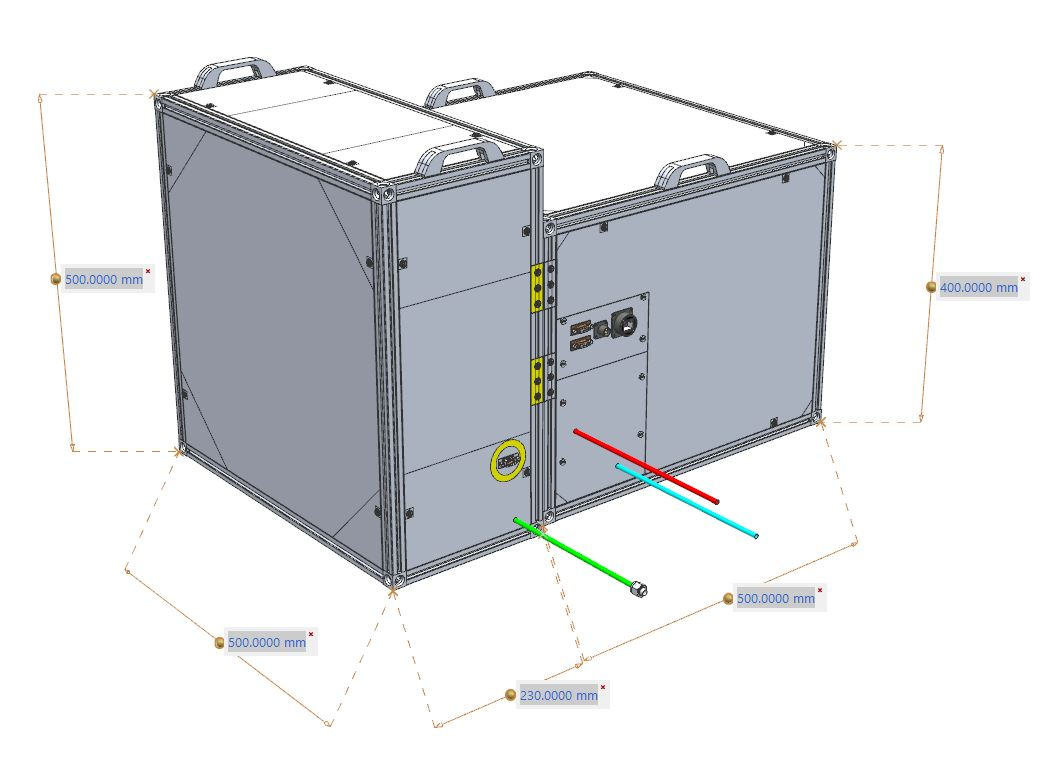
\includegraphics[width=0.9\textwidth]{4-experiment-design/img/Mechanical/tubular_dimensions.jpg}
     \caption{General Dimensions of the Experiment.}
     \label{dimensions}
\end{figure}

\begin{figure}[H]
    \centering
    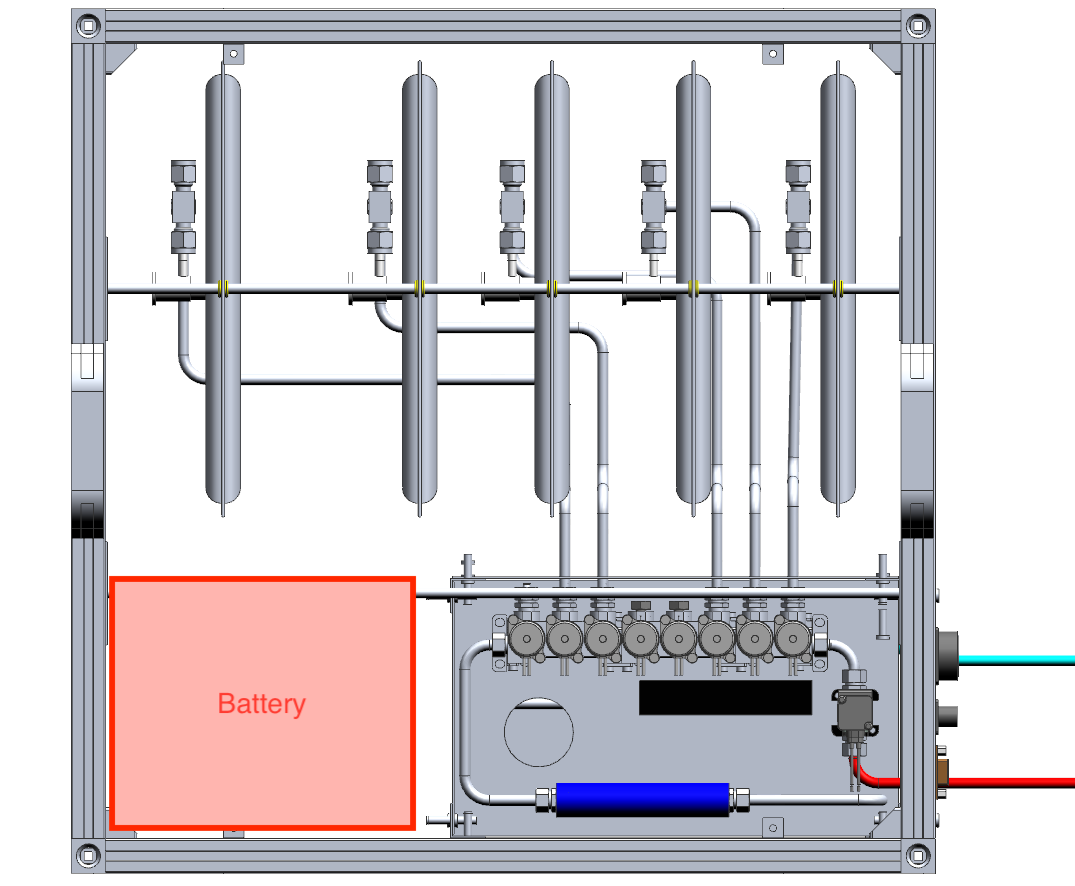
\includegraphics[width=0.45\textwidth]{4-experiment-design/img/Mechanical/Battery_Top_View.png}
    \caption{Layout Including a Battery (in Red).}
    \label{battery_distribution}
\end{figure}

The main mechanical characteristics of the experiment are summarized in Table \ref{table:experiment-summary}, where the values are based on the reference axis shown in Figure \ref{COG}. The Center Of Gravity for the whole experiment is determined to be located just on base of the third level of The Brain which coincides with the location of the electronics PCB. This outcome is quite advantageous in terms of stability for one of the most sensitive subsystems of the experiment in terms of shakes and loads. It should also be noted that the weights of the table for the boxes and, therefore, the whole experiment, are increased by a safety margin of $10\%$.

\begin{table}[H]
\noindent\makebox[\columnwidth]{%
\scalebox{0.8}{
\begin{tabular}{c|c|c|c|}
\cline{2-4}
 & CAC & AAC & TOTAL \\ \hline
\multicolumn{1}{|c|}{Experiment mass {[}kg{]}} & $12.08$ & $12.37$ & $24.45$ \\ \hline
\multicolumn{1}{|c|}{Experiment dimensions {[}m{]}} & $0.23\times0.5\times0.5$ & $0.5\times0.5\times0.4$ & $0.73\times0.5\times0.5$ \\ \hline
\multicolumn{1}{|c|}{Experiment footprint area {[}m^2{]}} & $0.115$ & $0.25$ & $0.365$ \\ \hline
\multicolumn{1}{|c|}{Experiment volume {[}m^3{]}} & $0.0575$ & $0.1$ & $0.1575$ \\ \hline
\multicolumn{1}{|c|}{Experiment expected COG position} & \begin{tabular}[c]{@{}l@{}}$X=23.51\ cm$\\ $Y=10\ cm$\\ $Z=22.57\ cm$ \end{tabular}  & \begin{tabular}[c]{@{}l@{}} $X=29.04\ cm$\\ $Y=16.63\ cm$\\  $Z=16.2\ cm$ \end{tabular} &\begin{tabular}[c]{@{}l@{}} $X=26.31\ cm$\\ $Y=24.99\ cm$\\  $Z=19.35\ cm$  \end{tabular} \\ \hline
\end{tabular}}}
\caption{Experiment Summary Table.}
\label{table:experiment-summary}
\end{table}


 \begin{figure}[H]
     \centering
     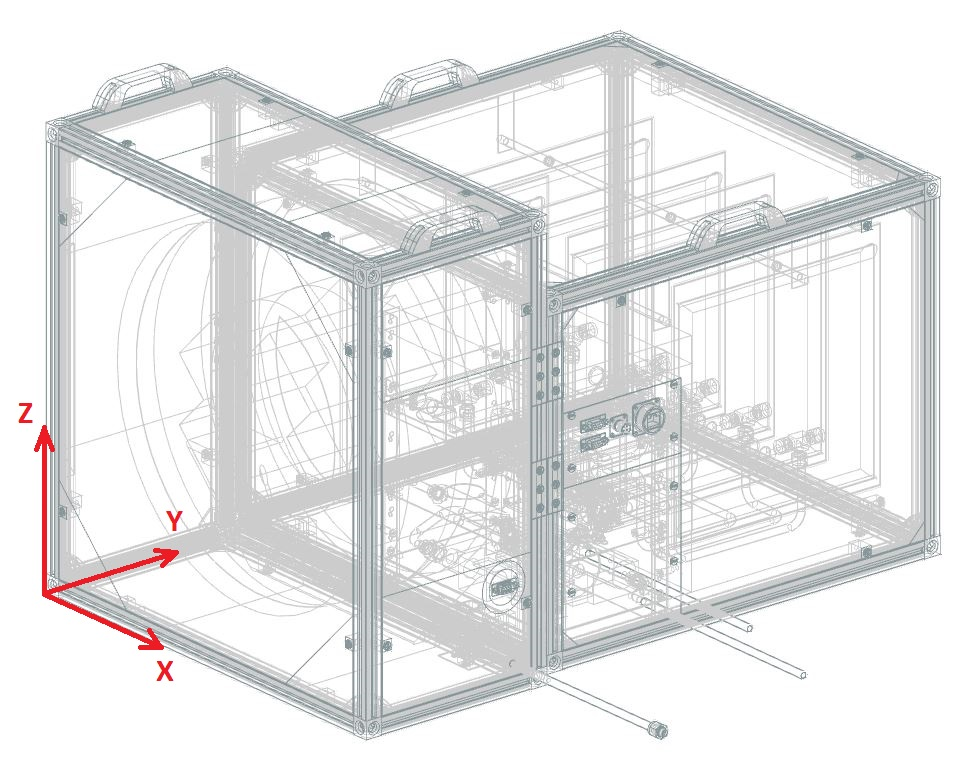
\includegraphics[width=0.45\textwidth]{4-experiment-design/img/Mechanical/COG.jpg}
     \caption{Reference Axis for the Total Center of Gravity.}
     \label{COG}
\end{figure}

\pagebreak
\subsubsection{Structure}
\label{sec:4.4.1}

The main purpose of an experiment box structure is to provide overall mechanical integrity and maintain the system geometry. It shall be able to carry the loads of all the phases of the flight and ensure that all the components and subsystems can withstand them. Test 9 in Table \ref{tab:vibration-test} will help to confirm the frame can withstand these vibrations and updates to the design will be made if necessary.

Moreover, other considerations such as electrical and, especially, thermal conductivity are also be a concern since the experiment will fly up to $25\ km$ in the Polar Circle in October and many critical subsystems have tight operative ranges values.

 \begin{figure}[H]
     \centering
     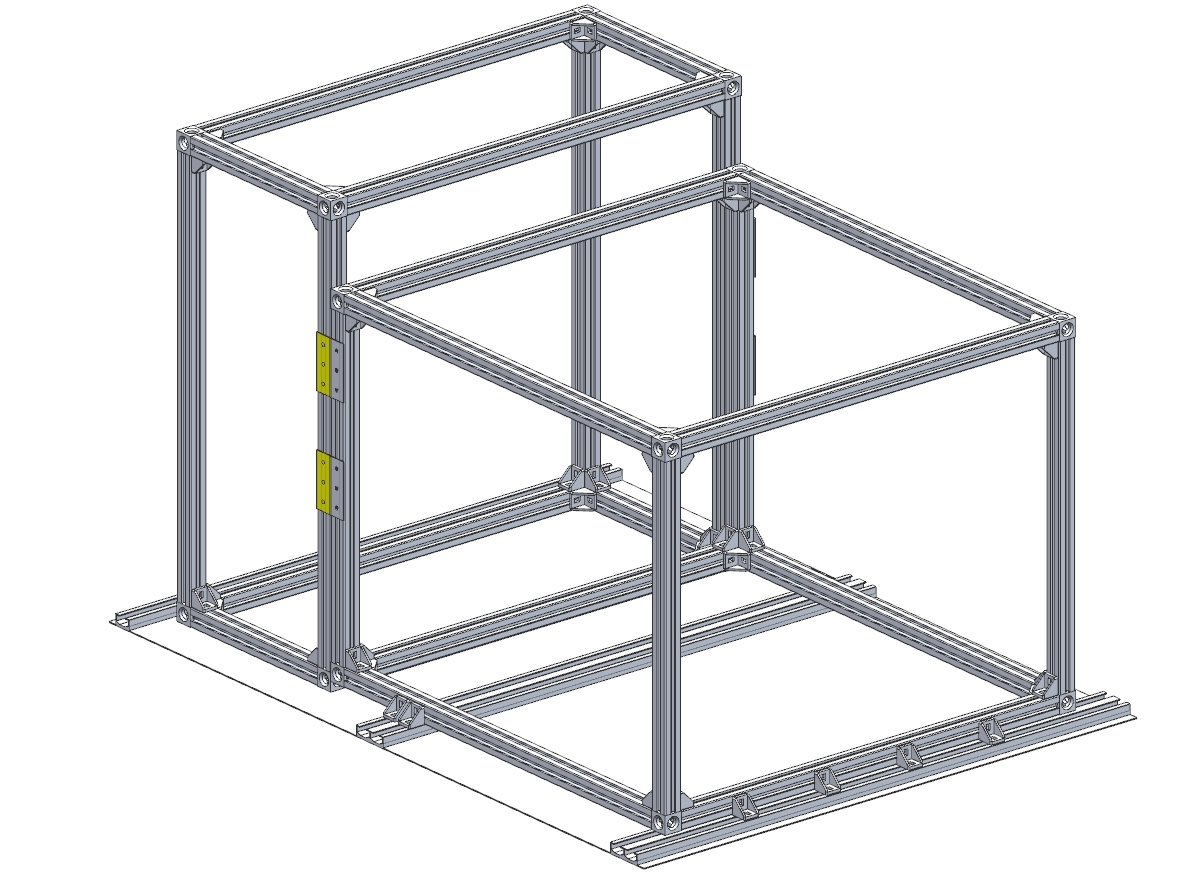
\includegraphics[width=0.8\textwidth]{4-experiment-design/img/Mechanical/structure_pic.jpg}
     \caption{Structure Overview.}
     \label{fig:structure}
\end{figure}

For this purpose, two boxes built with straight frames have been chosen as the best option as shown in Figure \ref{fig:structure}. The frame of these boxes will be strut profiles made of aluminum, with a characteristic cross-section of $20\times20\ mm$, and with $M6$ thread at each side. The rails will allow an easy interface between bars and other elements. In turn, these profiles will be joined together in each corner with aluminum cubic connectors of $20\times20\ mm$ (see Figure \ref{fig:corner_cube}) and $M6\times16$ bolts aligned with the bars axis. At the same time, these nodes will be reinforced by three $20/20$ brackets (see Figure \ref{fig:corner_bracket}) each that will be fixed to the frames with $M4\times8$ bolts and the corresponding $M4$ T-nut.

\bigskip
\begin{figure}[H]
    \noindent\makebox[\textwidth]{%
    \begin{subfigure}{.35\textwidth}
        \centering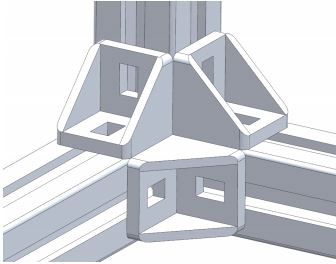
\includegraphics[width=1\textwidth]{4-experiment-design/img/Mechanical/corner_brackets.jpg}
        \caption{Brackets Reinforcement.}
        \label{fig:corner_bracket}
    \end{subfigure}
    \hspace{1cm}
    \begin{subfigure}{.35\textwidth}
        \centering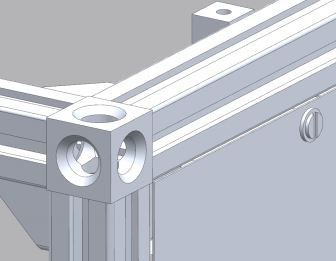
\includegraphics[width=1\textwidth] {4-experiment-design/img/Mechanical/corner_cube.jpg}
        \caption{Cubic Connector.}
        \label{fig:corner_cube}
    \end{subfigure}}
    \caption{Strut Profiles Connections.}
    \label{fig:profile_connection}
\end{figure}

\bigskip
Tables \ref{table:profile_material} and \ref{table:profile_momentum} below show the main mechanical properties of the Bosch Rexroth $20/20$ strut profiles used in the structure.


\begin{longtable}{|m{0.2\textwidth}|m{0.14\textwidth}|m{0.25\textwidth}|m{0.3\textwidth}|}
\hline
\textbf{Section surface} & \textbf{Mass} & \textbf{Moment of Inertia ($I_x = I_y$)} & \textbf{Moment of resistance ($W_x = W_y$)} \\ \hline 
$1.6\ cm^2$ & $0.4\ kg/m$ & $0.7\ cm^4$ & $0.7\ cm^3$ \\ \hline

\caption{Intrinsic Characteristics of the Strut Profiles.}
\label{table:profile_momentum}
\end{longtable}

\smallskip

\subsubsection{Walls and Protections}
\label{sec:4.4.2}

Since the experiment will be placed close to the outside of the gondola, it is very exposed to both external elements impacts and also possible broken parts from other experiments in the gondola due to unexpected rapid movements, and a probable hard landing impact. Therefore, the experiment box will be shielded with removable aluminum walls along with a thick layer of Styrofoam attached to each wall. This thickness varies from two to three centimeters in the AAC box, and five centimiters to protect the AirCore. Besides protection, the thickness of the styrofoam is also motivated by thermal control issues.
% which is explained more in detail in Section \ref{sec:4.6.6}.

To mount the experiment a combination of three different elements will be used, as shown in Figure \ref{fig:wall_attach}. The walls will be screwed to the Variofix blocks by means of $M4\times8$ bolts. In between the aluminum walls and the bolts, a $M4$ retainer ring will be placed to improve the fixation of each spot. Four fixation points for each wall have been considered sufficient to keep the experiment safe from any impact. However, double the amount of fixation points, eight, will be used in the more exposed walls that are facing outside the gondola.

The styrofoam sheets will be attached to the aluminum walls with polyamide washers screwed along both layers.

Tables \ref{table:wall_aluminum} and \ref{table:wall_styrofoam} show the main properties of the materials used to build the walls of the boxes.

 \begin{figure}[H]
     \centering
     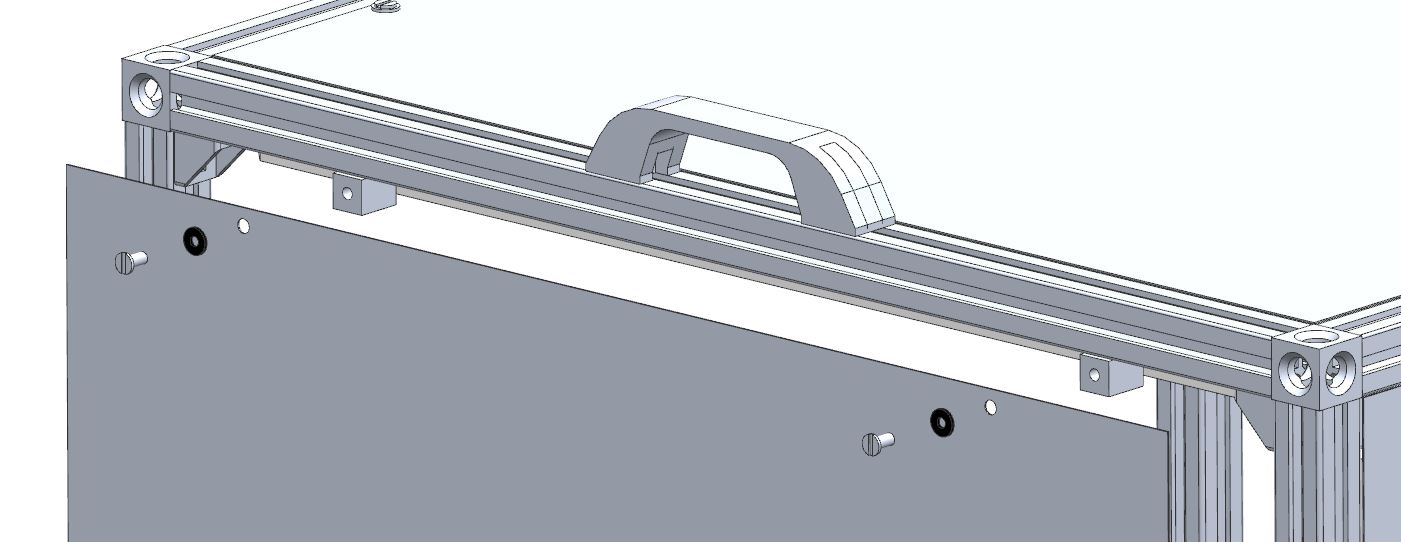
\includegraphics[width=0.8\textwidth]{4-experiment-design/img/Mechanical/wall_attachment.jpg}
     \caption{Exploit View of the Attachment of the Walls.}
     \label{fig:wall_attach}
\end{figure}

\subsubsection{CAC Box}

The CAC subsystem is designed to fit a $300$ m stainless steel coiled tube, a solenoid valve controlling it, interfaces, an air filter and three temperature sensors. A schematic of this subsystem can be seen in Figure \ref{fig:CAC-schematic}. The CAC consists of a combination of a $200$ m coiled tube of $1/8$ inches diameter and a $100$ m coiled tube of $1/4$ inches diameter. The outlet of the CAC is sealed with a quick connector provided by FMI. The inlet will be sealed the same way but it will be opened by another interface plugged into the quick connector. A filter is placed between this orifice and the solenoid valve. The filter will be custom made by FMI. The set up is a tube containing magnesium perchlorate powder with stone wool at both ends of the tube. It will ensure that no moisture will enter the coil during any testing or sampling. Another tube is attached to the solenoid valve that goes outside the box, thus having a direct outside outlet and inlet for the whole CAC system, as seen in Figure \ref{fig:CAC-cad-model}.

% mechanical issues and gondola constraints 

\begin{figure}[H]
    \centering
    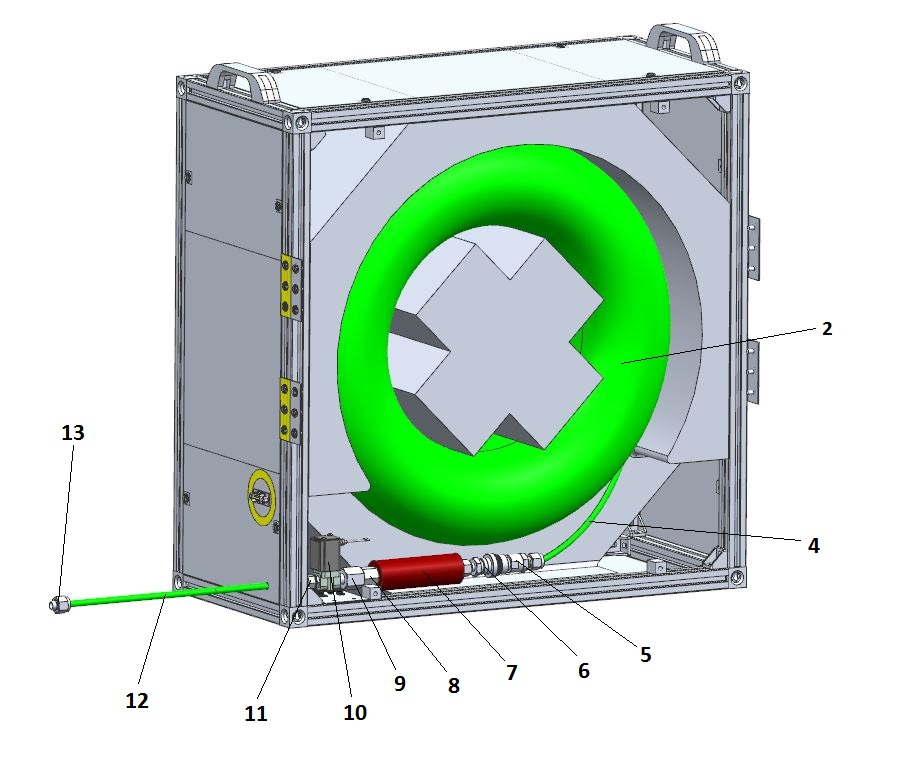
\includegraphics[width=0.7\textwidth]{4-experiment-design/img/Mechanical/CAC_interior_labels.jpg}
    \caption{3D Model of the CAC Box. The Numbers Correspond to the Numbers in Figure. \ref{fig:CAC-schematic}.}
    \label{fig:CAC-cad-model}
\end{figure}

\begin{figure}[H]
    \centering
    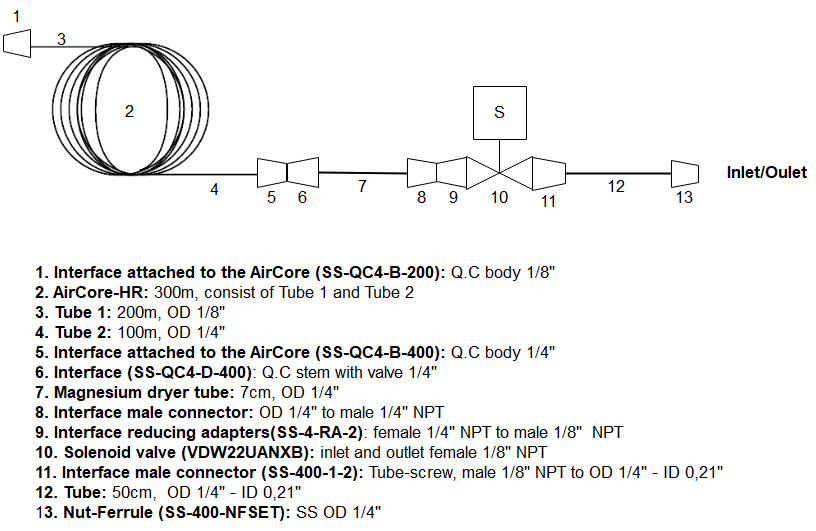
\includegraphics[width=1\textwidth]{4-experiment-design/img/Mechanical/CAC-schematic.PNG}
    \caption{Schematic of CAC.}
    \label{fig:CAC-schematic}
\end{figure}
\smallskip
The electronic components in the CAC box will be: three temperature sensors and the solenoid valve. In order to connect these components to the control unit in the AAC box, a D-sub cable will link the respective D-sub connector on each box.

\subsubsection{AAC Box}\label{sec:aac-analysis}
The AAC box has been designed to be as compact as possible. An analysis regarding the variation of the bags dimensions to different sampled volume, has been made and summarized in Appendix \ref{dimensions-bags}. From these results it was shown that the AAC subsystem is able to fit six $3\ L$ sampling bags together The Brain that includes the pneumatic system and the electronic box. Each bag will have a dedicated valve in the Valve Center (VC) to allow emptying and filling processes as well as to close the bag when needed. The bags will be hanging from a bar that will be attached to the structure frame by two anchor points on the top. The distribution layout can be seen in Figures \ref{iso_aac} and \ref{lateral_aac}. 
 

%The AAC Subsystem consists of six $3\ L$ sampling bags. Each bag will have a dedicated valve in the Valve Center (VC) to allow emptying and filling processes as well as to close the bag when needed. The bags will be placed vertically and will have two anchor points: on the top through a  multiple anchor interface (see Figure \ref{anchor_bags}) and on the bottom by means of the tubes connecting them to the valves.

%% Several Figures of the top box with its inside elements: isometric, top view and front view.

%\begin{figure}[H]
%    \centering
%    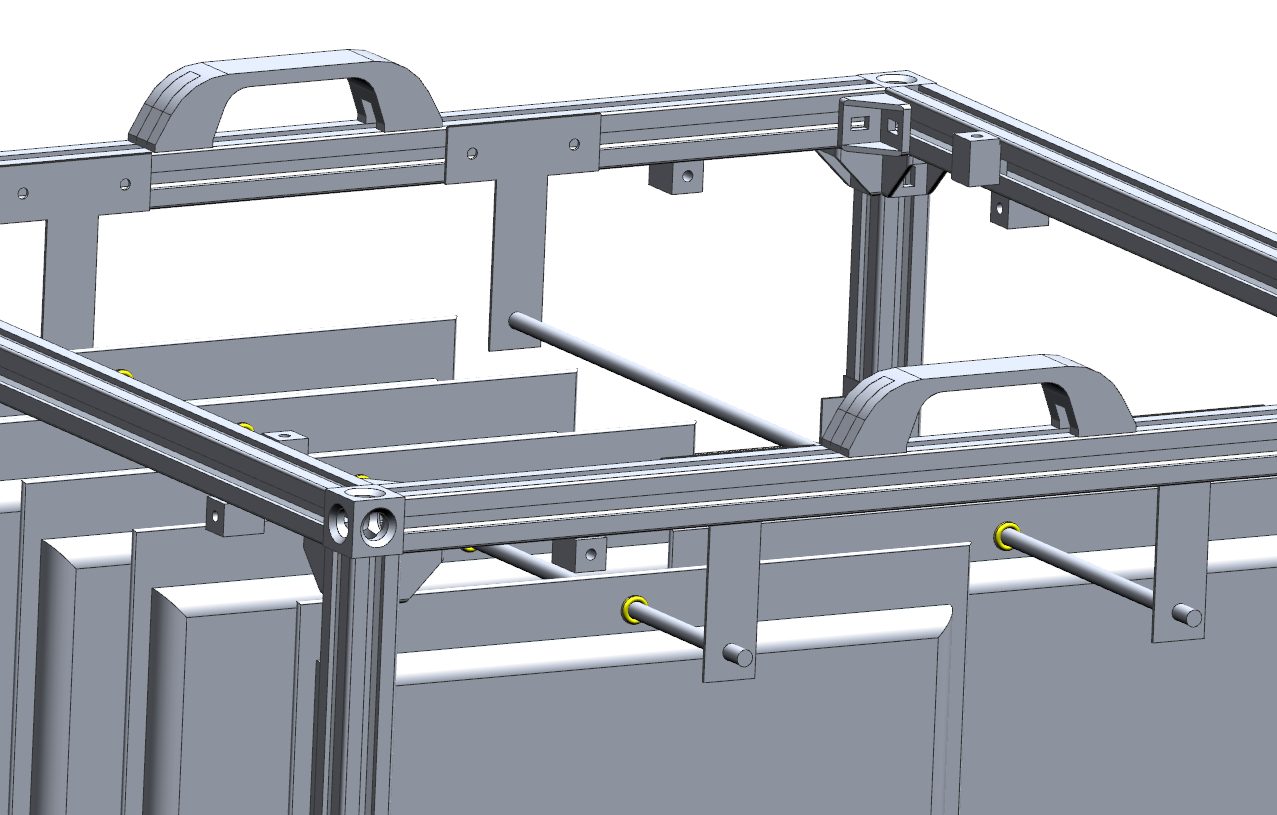
\includegraphics[width=0.6\textwidth]{4-experiment-design/img/Mechanical/Bags_Fixing_Interface.png}
%    \caption{Sampling Bags with Fixing Interface and the AAC Box Handles.}
%    \label{anchor_bags}
%\end{figure}


%\underline{Distribution}

%The AAC box has been designed to be as compact as possible, which was a challenging iterative process since the bags dimensions vary during the flight. The process led to a square base box that is able to fit six sampling bags together with a control center called The Brain that includes the pneumatic system and the electronic box. The distribution layout can be seen in Figures \ref{iso_aac} and \ref{lateral_aac}.

% Figure: Top view to show the distribution of the AAC Box

\begin{figure}[H]
    \centering
    \begin{subfigure}[b]{0.47\textwidth}
        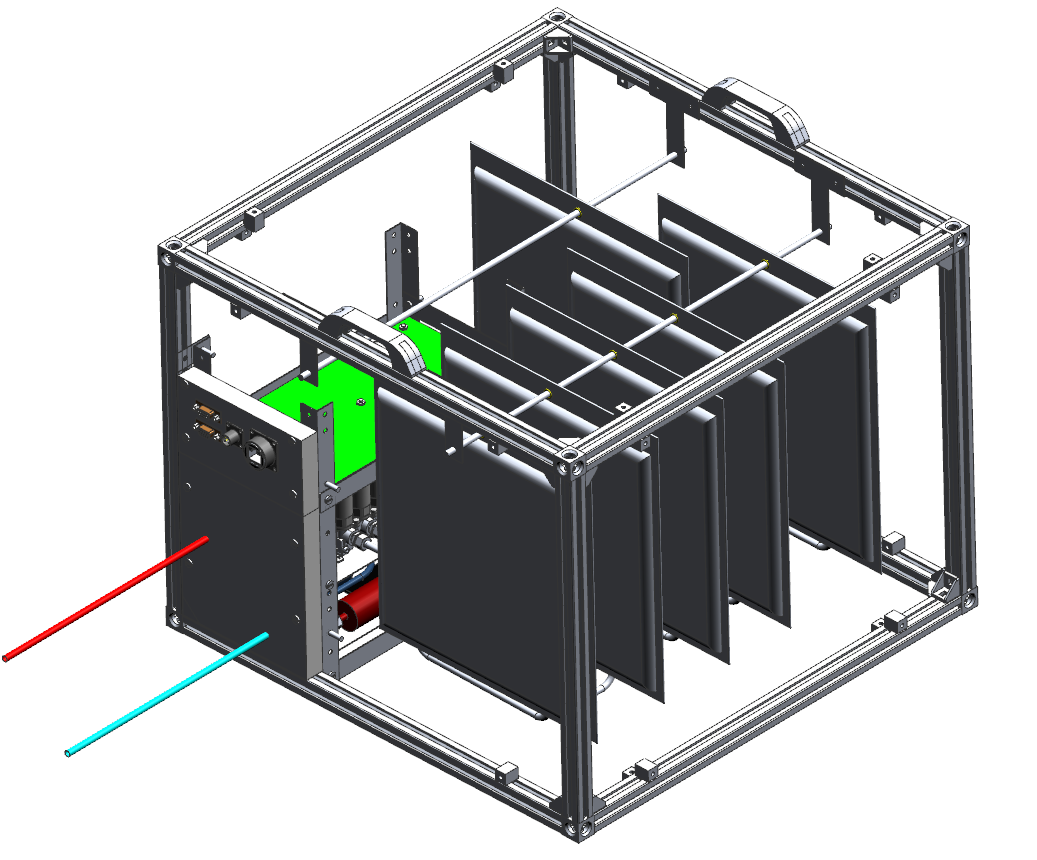
\includegraphics[width=\textwidth]{4-experiment-design/img/Mechanical/AAC_isometric_view.png}
         \caption{Isometric View of the AAC Box.}
    \label{iso_aac}
    \end{subfigure}
    ~
    \begin{subfigure}[b]{0.47\textwidth}
        \centering
         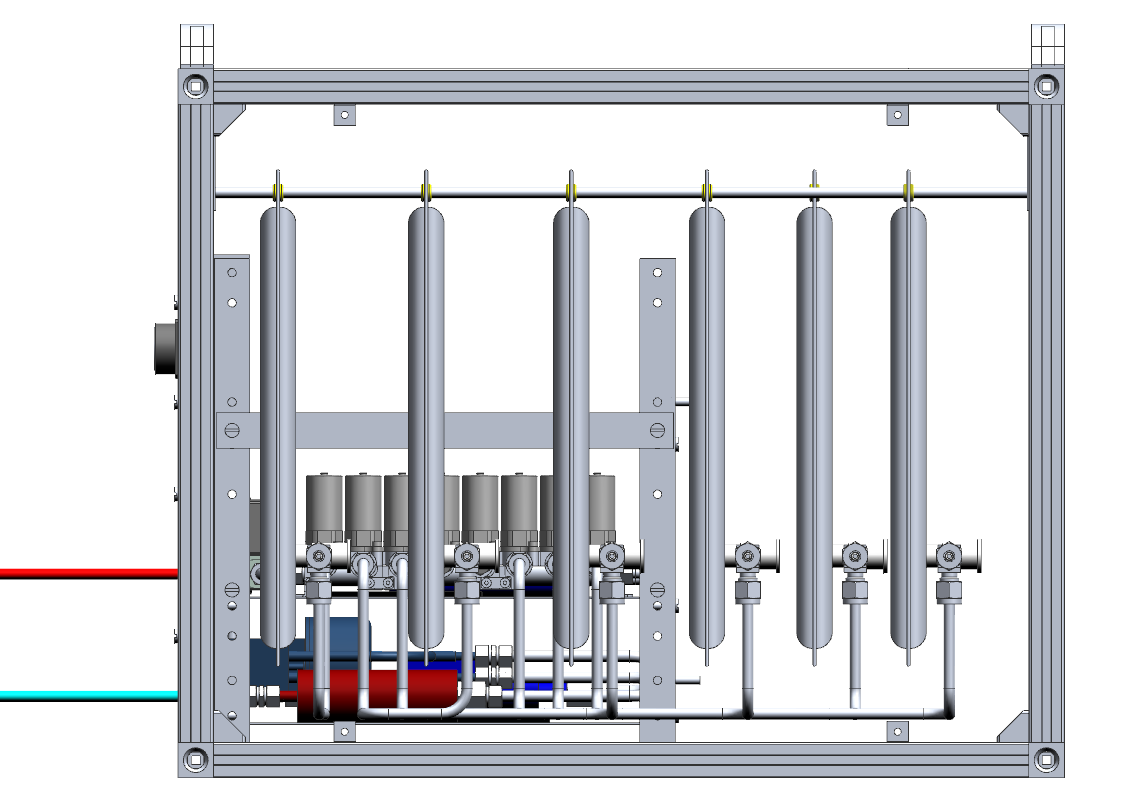
\includegraphics[width=\textwidth]{4-experiment-design/img/Mechanical/AAC_lateral_view.png}
        \caption{Lateral View of the AAC Box.}
        \label{lateral_aac}
        \end{subfigure}
    \caption{Distribution Inside the AAC Box.}
    \label{fig:Distribution-AAC}
\end{figure}

%\begin{figure}[H]
%    \centering
%    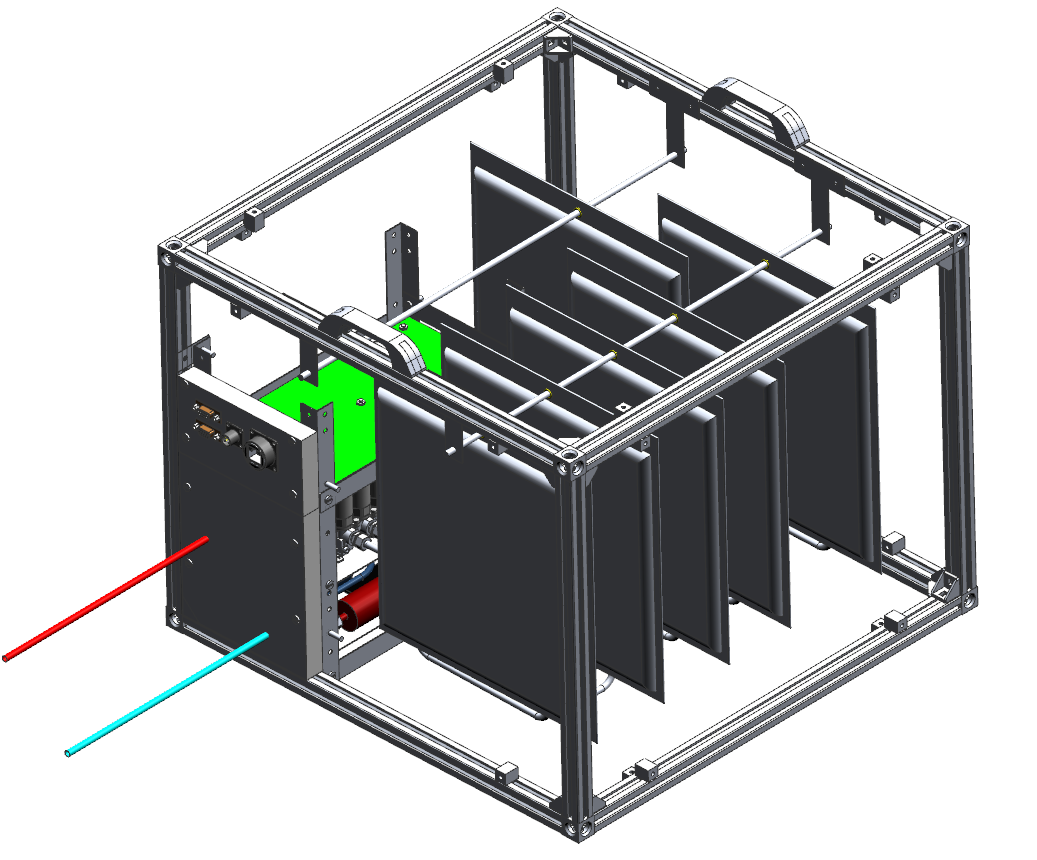
\includegraphics[width=0.6\textwidth]{4-experiment-design/img/Mechanical/AAC_isometric_view.png}
%    \caption{Isometric View of the AAC Box.}
%    \label{iso_aac}
%\end{figure}

%%\begin{figure}[H]
%    \centering
%    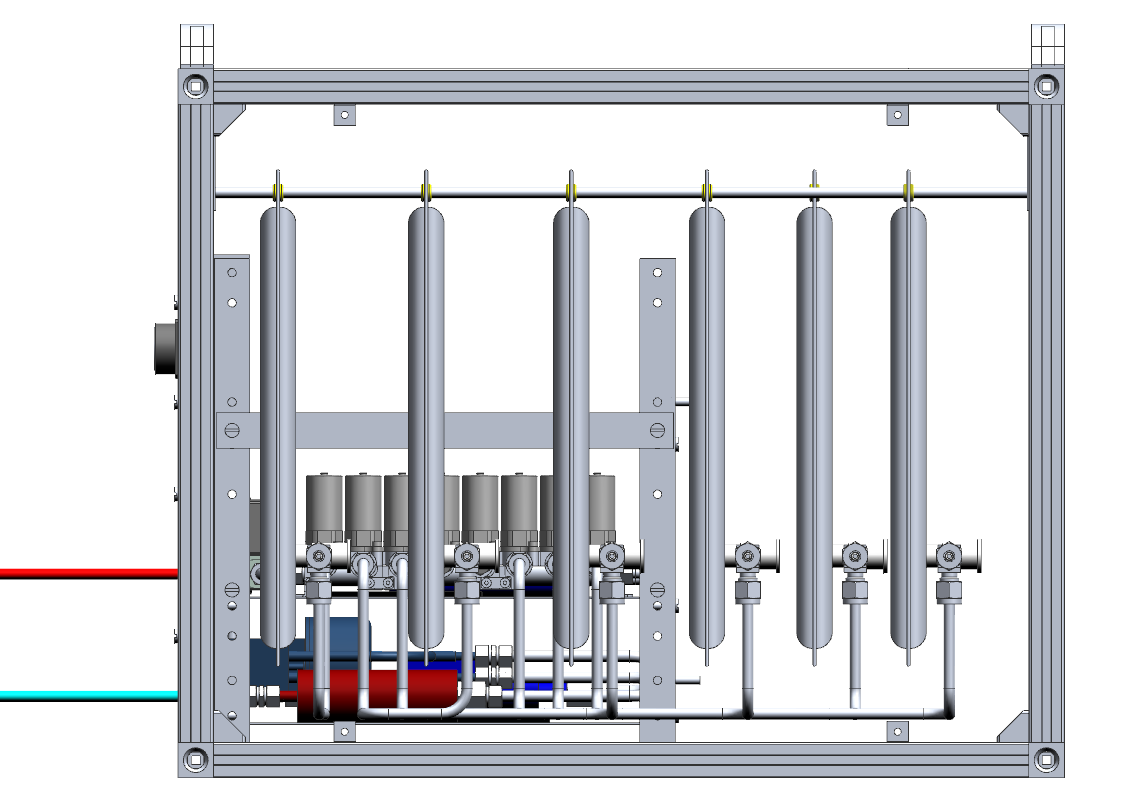
\includegraphics[width=0.6\textwidth]{4-experiment-design/img/Mechanical/AAC_lateral_view.png}
%    \caption{Lateral View of the AAC Box.}
%    \label{lateral_aac}
%\end{figure}

%\begin{figure}[H]
%    \centering
%    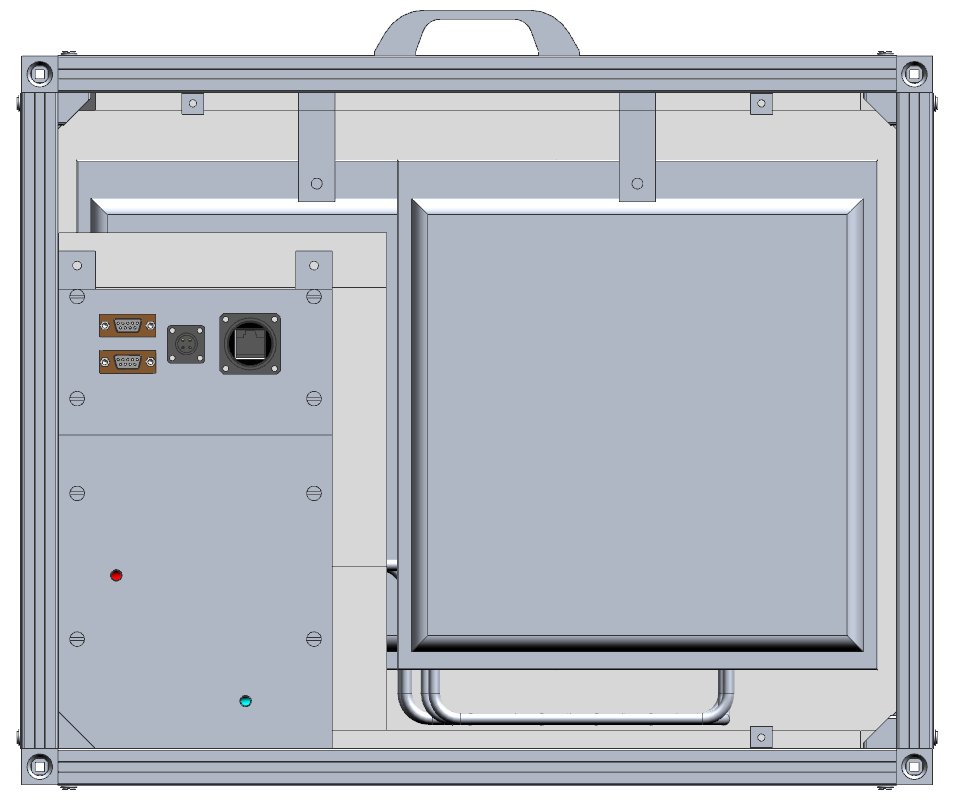
\includegraphics[width=0.7\textwidth]{4-experiment-design/img/Mechanical/AAC_front_view.png}
%    \caption{Front View of the AAC Box.}
%    \label{front_aac}
%\end{figure}
In order to reach to all the bags from the Valve Center, the tubes are brought to the base of the box. More detail on its positioning is included in the following section. 
%Since the AAC box is expected to be handed over to FMI, the design also takes into consideration the possibility to include a battery for power supply. This would be allocated next to The Brain and imply reducing the sampling bags down to five, see Figure \ref{battery_distribution}.

% Figure with a a top view without the 6th bag and with a red box simulating the battery

\bigskip
\underline{The Brain}
\label{subsec:brain}

\smallskip
The Brain is an essential part of the experiment. It is a three-level structure containing both the pneumatic system and the electronics of the experiment, seen in Figure \ref{brain_isometric_open}. Its design aimed to make it compact enough to both allow a proper thermal control and to fit into the space left next to the sampling bags. It is placed in a corner of the AAC box. Therefore, The Brain takes advantage of the vertical space inside the AAC box. It has three different levels: Level 1 - Pump, Level 2 - Valve Center and Level 3 - Electronics.


\begin{figure}[H]
    \centering
    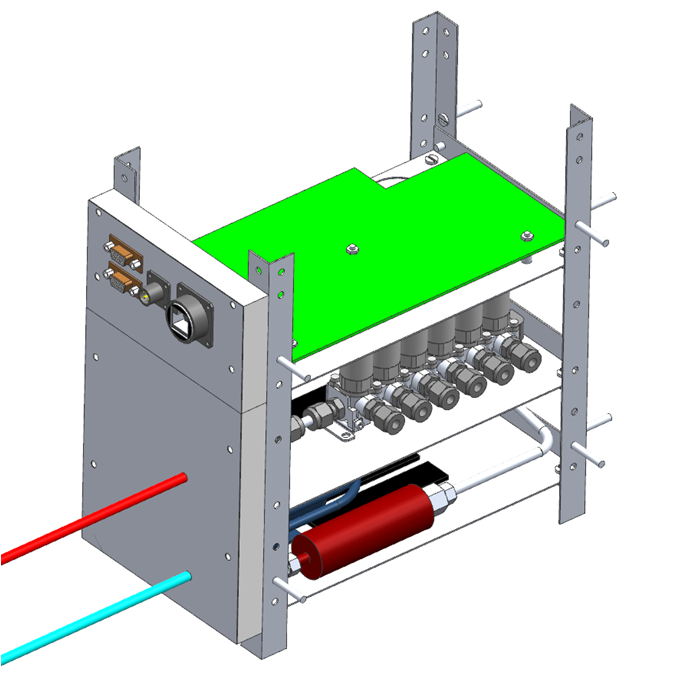
\includegraphics[width=0.43\textwidth]{4-experiment-design/img/Mechanical/The_Brain_Isometric.png}
    \caption{Isometric View of The Brain.}
    \label{brain_isometric_open}
\end{figure}
Level 1 of The Brain is lying on the base wall styrofoam. It contains the beginning of the pneumatic sampling system. The inlet tube passes through the wall and interfaces with the filter. From here the system continues through the pump, airflow sensor and to Level 2. The reason for having the pump in Level 1 is to have the minimum vibration transmitted to the other components. The pump will have two heaters close by that will be used to regulate its temperature. This can be seen as two black rectangular sheets underneath the pump in Figure \ref{level_1}.

The second level of The Brain is responsible for the distribution of the air to the selected sampling bag. The manifold with 8 solenoid valves is the main component. From here, the tubes connect with the bags. A T-Union connection is used just before the bag valve. This interface allows the pre-flight flushing of the tubes connecting with the valves as explained previously. 

\smallskip
The flushing valve is the responsible to ensure a proper flushing of the system before each sampling period. From the flushing valve, a outlet tube (in red) reaches the outside environment. This can be seen in Figure \ref{level_2}.

The OBC and its external elements will be allocated in the third level of The Brain. The PCB will be fixed to the aluminum plate by means of 5 standoffs. As shown in Figure \ref{level_3}, it has a hole, as well as the level plate, to collect all the wires connecting with levels 1 and 2. This level has its own outside wall which contains the electrical interfaces. The latter allows to open the wall without having to remove all the sockets attached with screws and a female in the inside of the wall. The styrofoam shielding of The Brain has a hole at this height to allow the temperature sensors wires to reach the inside of the AAC Box. 

A more detailed content of the components for each level is summarized in Appendix \ref{list-of-components-brain}.
\begin{figure}[H]
    \centering
    \begin{subfigure}[b]{0.3\textwidth}
    \centering
    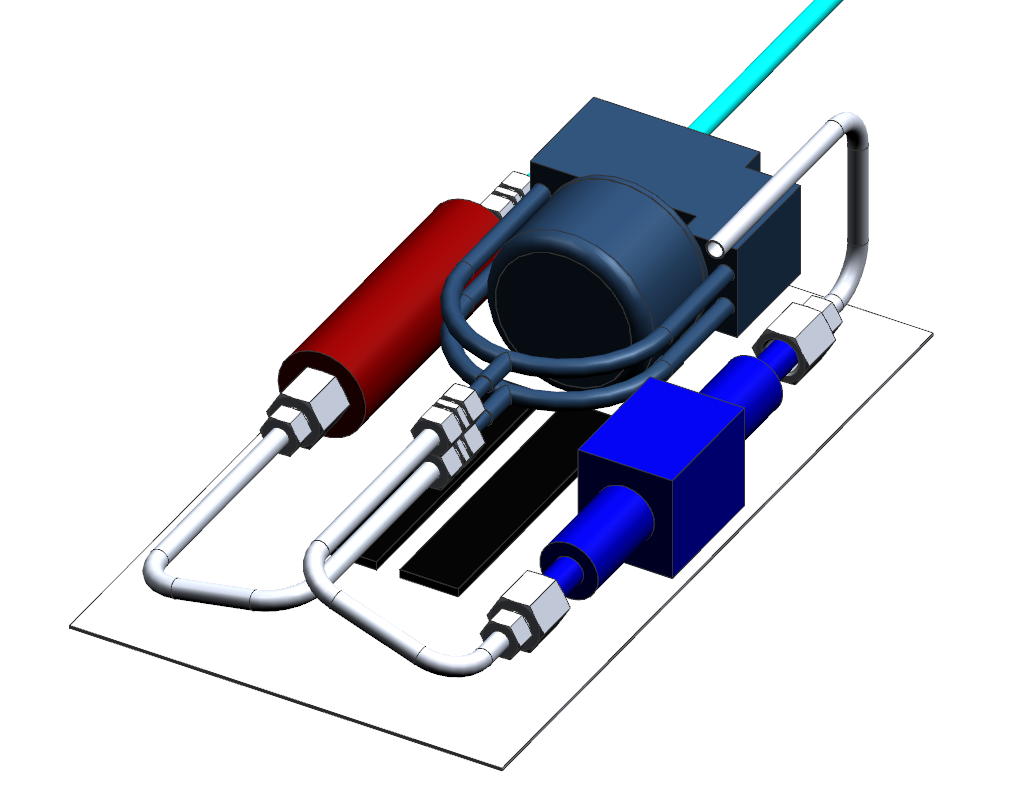
\includegraphics[width=\textwidth]{4-experiment-design/img/Mechanical/Level_1.png}
    \caption{Isometric View of Level 1.}
    \label{level_1}
    \end{subfigure}
    ~
    \begin{subfigure}[b]{0.3\textwidth}
    \centering
    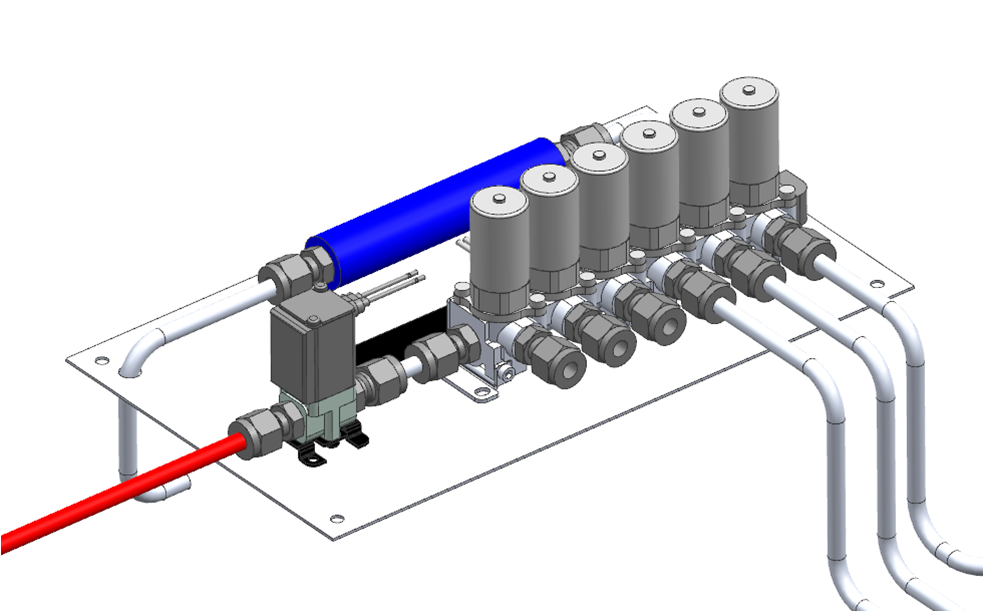
\includegraphics[width=\textwidth]{4-experiment-design/img/Mechanical/Level_2.png}
    \caption{Isometric View of Level 2.}
    \label{level_2}
    \end{subfigure}
    ~
    \begin{subfigure}[b]{0.3\textwidth}
    \centering
    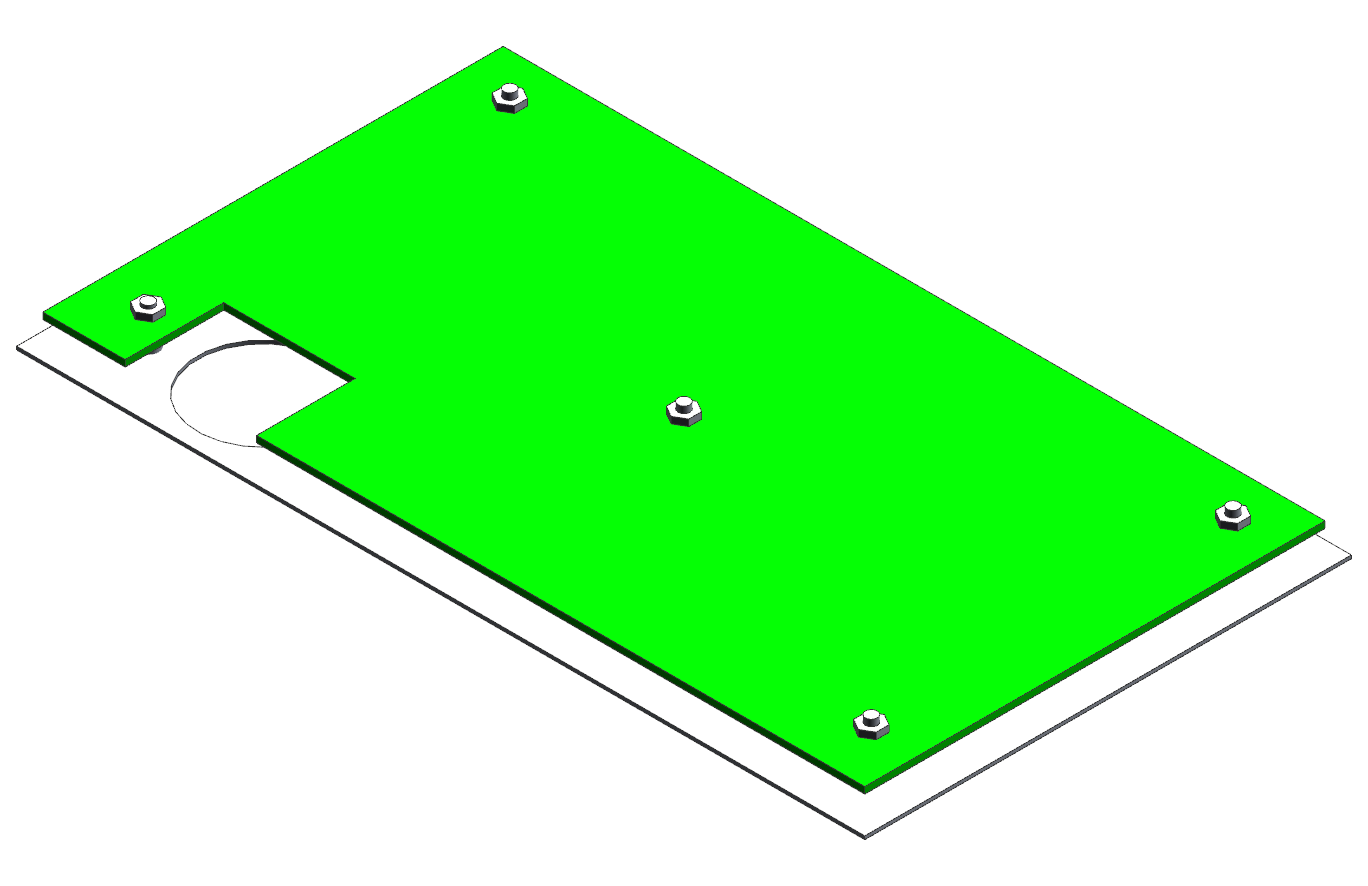
\includegraphics[width=\textwidth]{4-experiment-design/img/Mechanical/Level_3.png}
    \caption{Isometric View of Level 3.}
    \label{level_3}
    \end{subfigure}
    \caption{Distribution in Each Level.}
    \label{fig:The-brain}
\end{figure}
%Level 1 is the base of the AAC box and together with Level 2 contain the main pneumatic system. This is commanded by the electronics in the top level. This distribution allows easy access to the PCB from the top and provides the physical desired separation between electronics and pneumatic circuit. 

This distribution allows easy access to the PCB from the bottom and provides the physical desired separation between electronics and pneumatic circuit.
%This is shown in the dedicated section for each level which can be seen in Figure \ref{brain_lateral}.

%\begin{figure}[H]
%    \centering
%    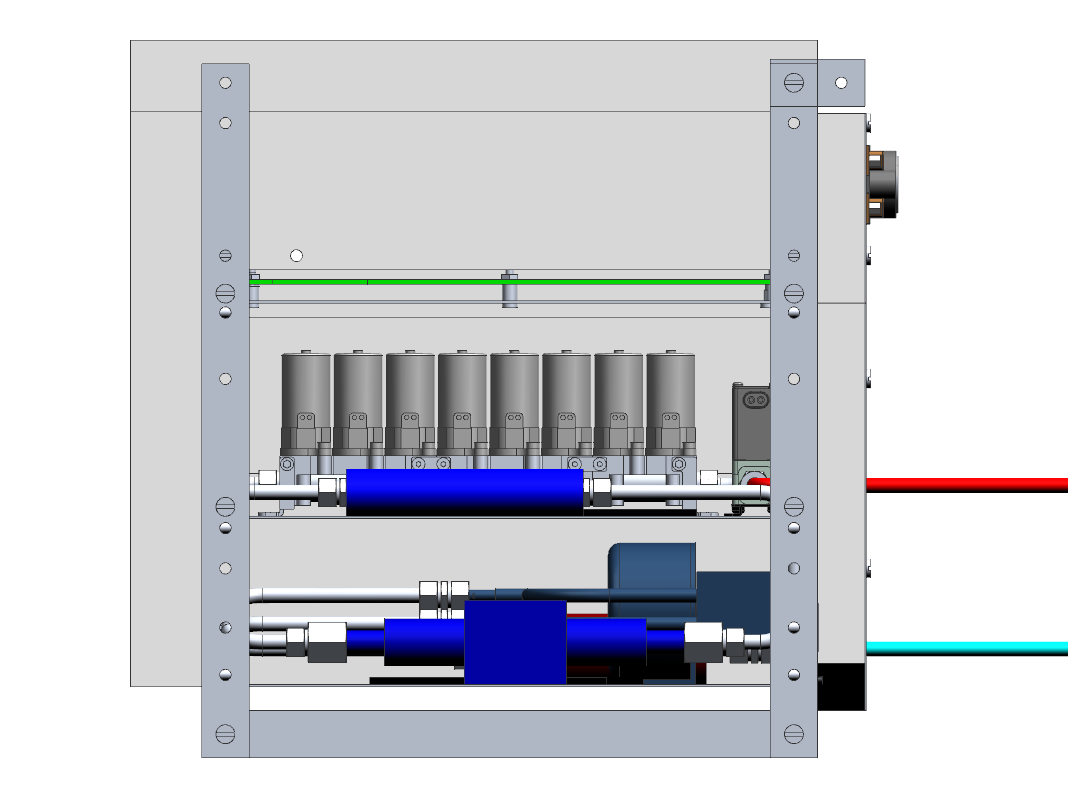
\includegraphics[width=0.6\textwidth]{4-experiment-design/img/Mechanical/Brain_Lateral.png}
%    \caption{Lateral View of The Brain.}
%    \label{brain_lateral}
%\end{figure}

\smallskip
The structure of The Brain provides versatility in terms of implementation and construction. It is made out of four aluminum 90-degree angle bars and five flat bars to join them together. The bars have custom-made holes that allow the 1 mm thick aluminum plate of each level to be fixed by means of two bolts on each column, one over and one below it. They allow the possibility to provide the anchor point for the lateral and top styrofoam shield as well as to fix the whole unit to the box structure bars. This is seen in Figure \ref{brain_structure}. 

\begin{figure}[H]
    \centering
    \begin{subfigure}[b]{0.48\textwidth}
    \centering
    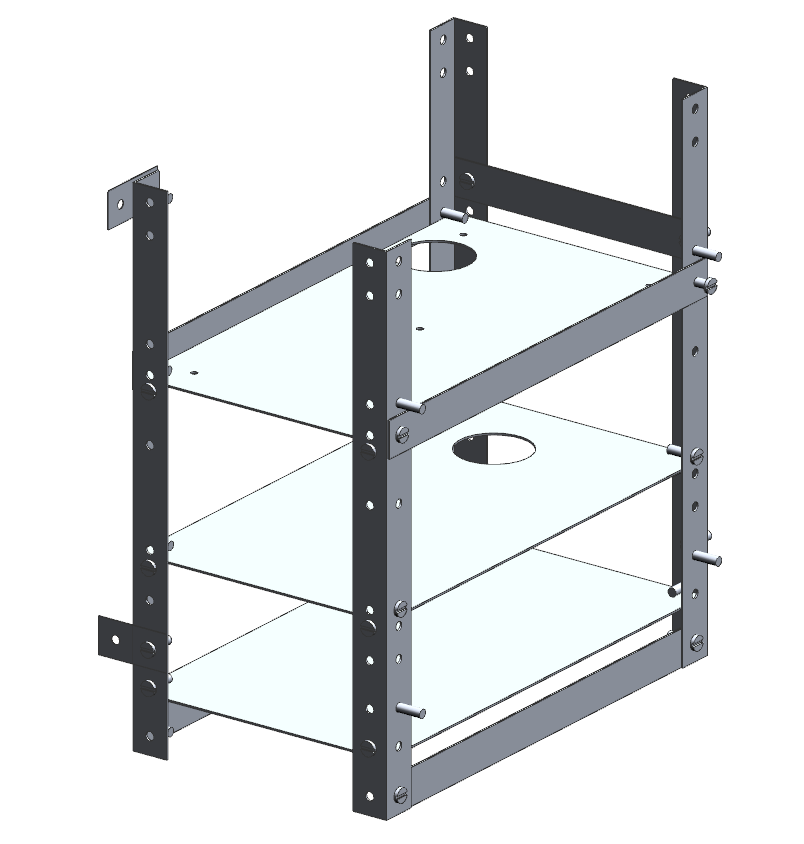
\includegraphics[width=\textwidth]{4-experiment-design/img/Mechanical/Brain_Structure.png}
    \caption{Structure of The Brain.}
    \label{brain_structure}
    \end{subfigure}
    ~
    \begin{subfigure}[b]{0.48\textwidth}
    \centering
    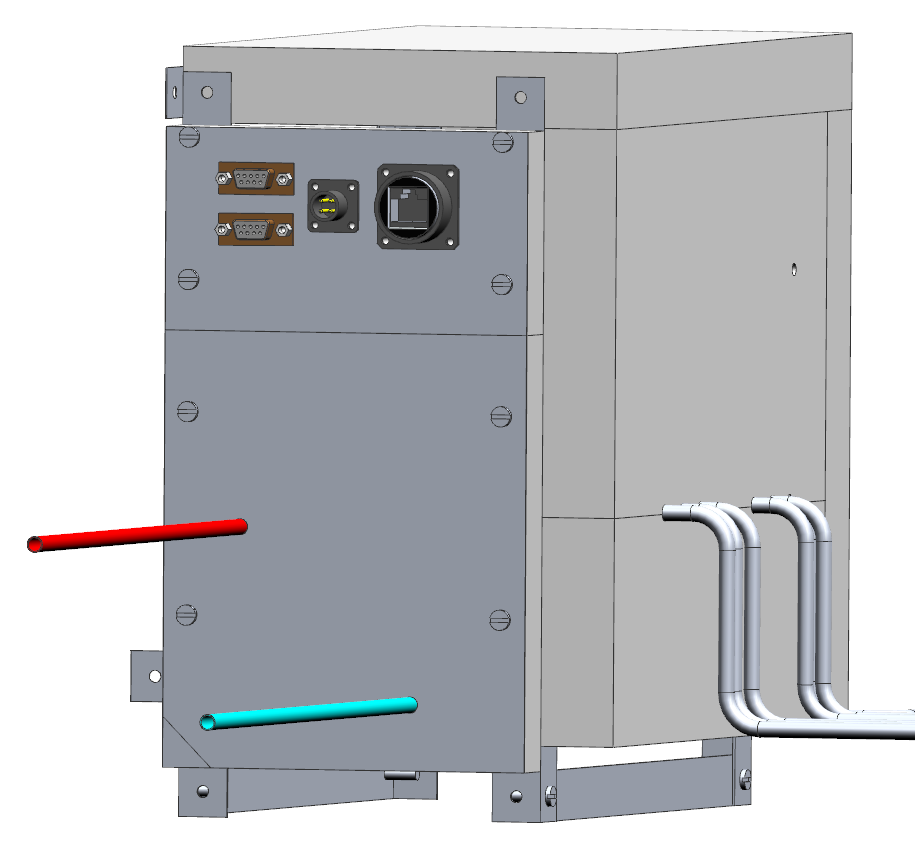
\includegraphics[width=\textwidth]{4-experiment-design/img/Mechanical/Brain_Isometric.png}
    \caption{Isometric View of The Brain with Walls.}
    \label{brain_isometric}
    \end{subfigure}
    \caption{Design of The Brain.}
    \label{fig:The-brain}
\end{figure}



%\begin{figure}[H]
%    \centering
%    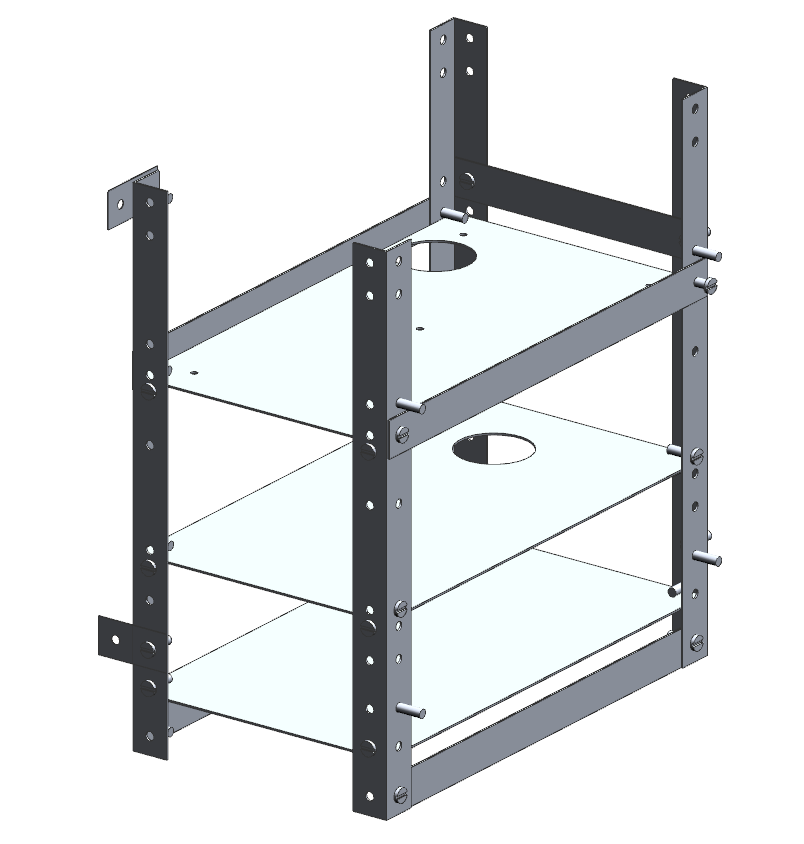
\includegraphics[width=0.8\textwidth]{4-experiment-design/img/Mechanical/Brain_Structure.png}
%    \caption{Structure of The Brain.}
%    \label{brain_structure}
%\end{figure}

\smallskip
The bulk dimensions of The Brain are 260 mm long, 150mm wide and 290 mm high. If the shielding styrofoam walls are taken into account, the dimensions are 290 mm long, 180 mm wide and 300 mm high.
Therefore, accounting for the space the column bars take, each plate has a surface of 258 mm x 158 mm. The distance between levels is variable depending on the components dimensions. Level 1 has a height if 7 cm, Level 2 has a height of 9 cm and Level 3 has 8 cm to the top styrofoam shielding. The Brain with styrofoam sheilding can be seen in Figure \ref{brain_isometric}.

%\begin{figure}[H]
%    \centering
%    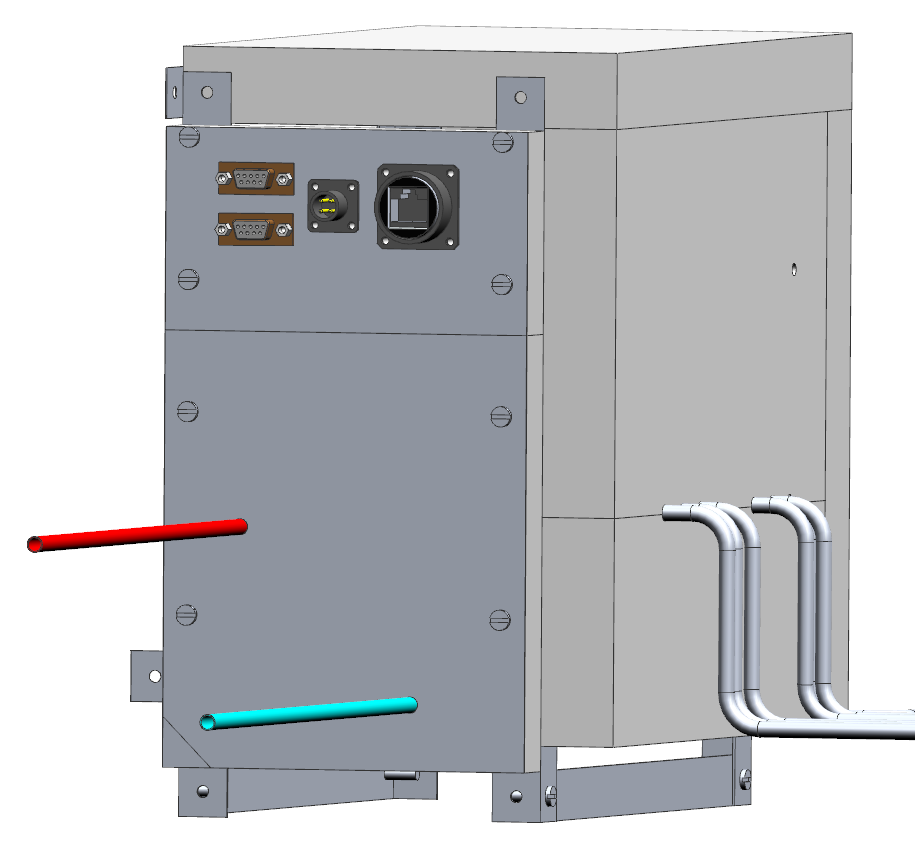
\includegraphics[width=0.8\textwidth]{4-experiment-design/img/Mechanical/Brain_Isometric.png}
%    \caption{Isometric View of The Brain.}
%    \label{brain_isometric}
%\end{figure}

\smallskip
In order to allocate the electrical interfaces required (E-Link, Power Supply and D-Sub Connectors) as well as to allow the tubes of the sampling system to reach the outside environment, the outside facing wall is divided in three pieces. Two small pieces of aluminium sheet are fixed to The Brain structure, as seen in Figure \ref{brain_isometric}. This will make it easy to manipulate when having to open the box wall since the little pieces containing the interfaces and the tubes holes, will remain attached. The bottom piece covers Level 1 and 2 while the other, which contains the electrical connections, protects Level 3. These pieces have the same layout as the main wall. 





%\begin{figure}[H]
%    \centering
%    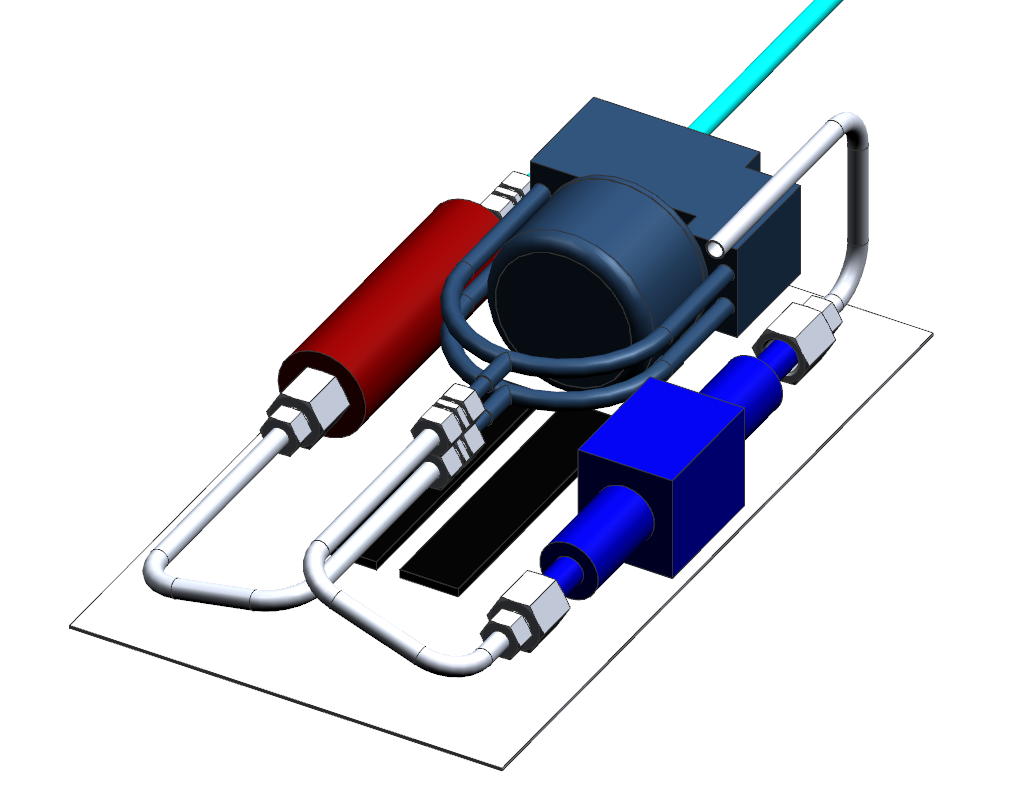
\includegraphics[width=0.8\textwidth]{4-experiment-design/img/Mechanical/Level_1.png}
%    \caption{Isometric View of Level 1.}
%    \label{level_1}
%\end{figure}


%\begin{figure}[H]
%    \centering
%    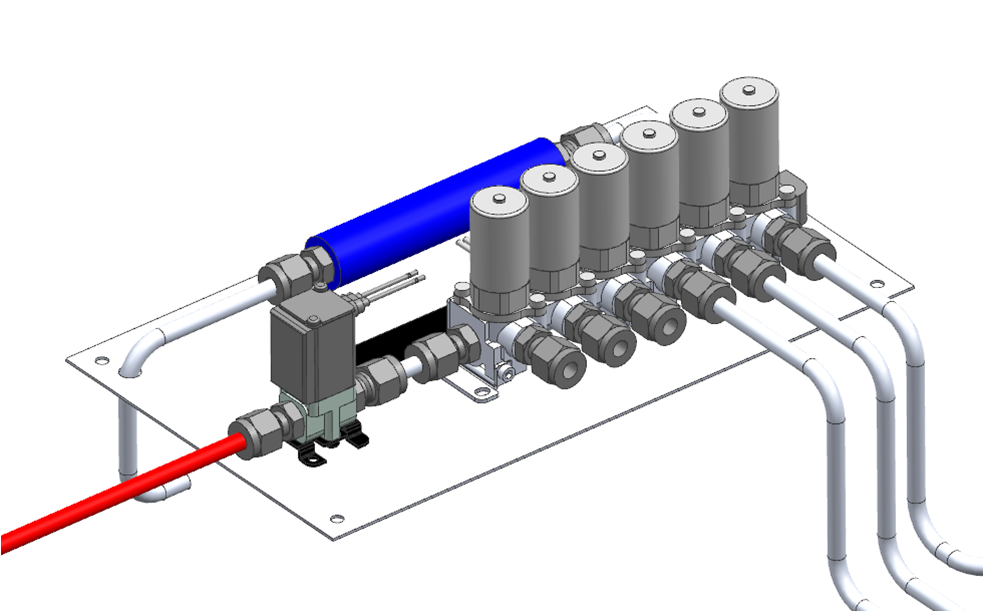
\includegraphics[width=0.8\textwidth]{4-experiment-design/img/Mechanical/Level_2.png}
%    \caption{Isometric View of Level 2.}
%    \label{level_2}
%\end{figure}



%\begin{figure}[H]
%    \centering
%    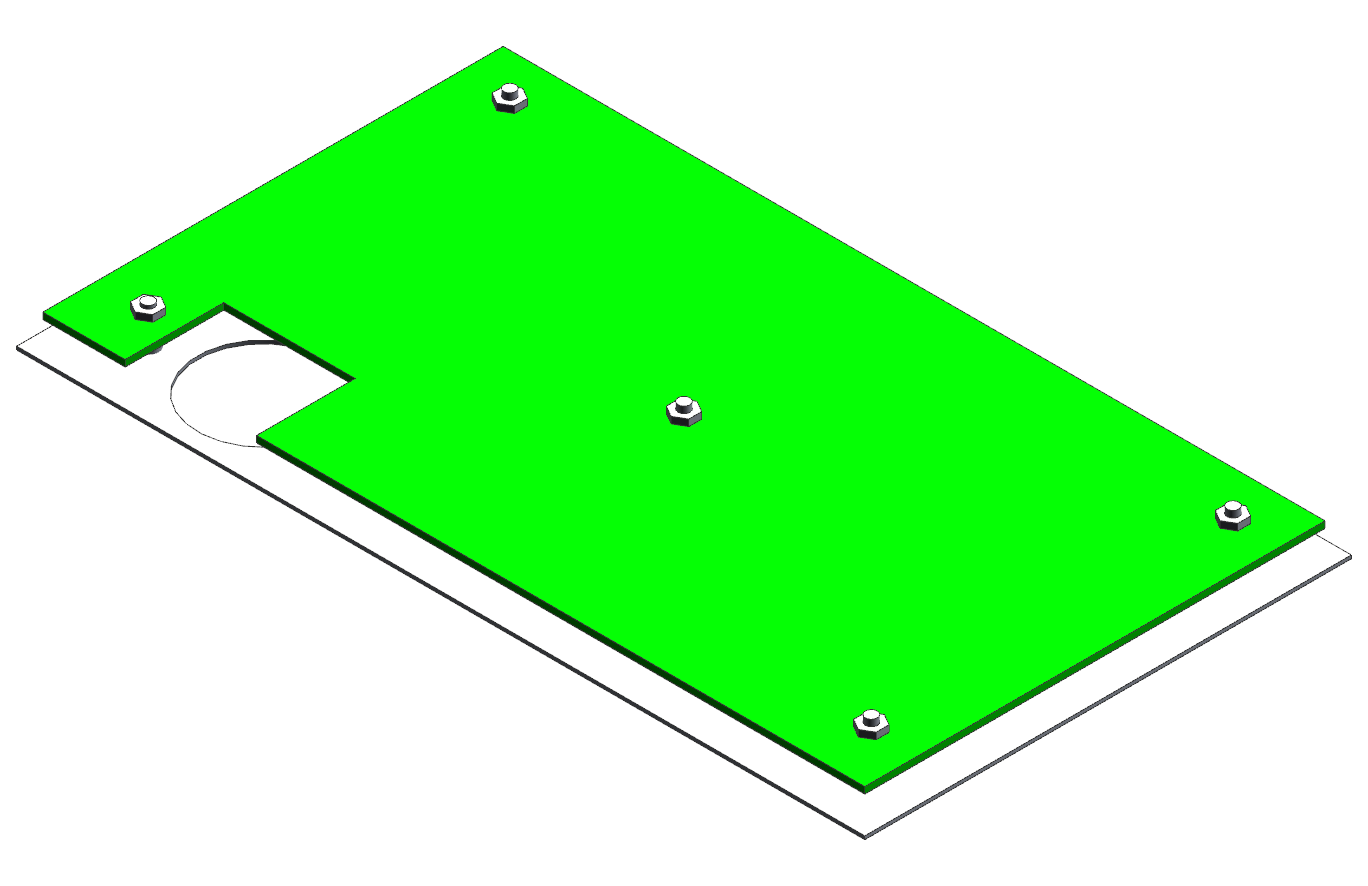
\includegraphics[width=0.8\textwidth]{4-experiment-design/img/Mechanical/Level_3.png}
%    \caption{Isometric View of Level 3.}
%    \label{level_3}
%\end{figure}

\bigskip
\underline{Shielding and anchor points}

\smallskip
The most critical components in terms of required thermal control are inside The Brain. These are the pump and the valves. In order to provide a passive thermal shielding, 3 cm thick removable styrofoam walls are placed in the three walls (top and laterals) facing the interior of the AAC box, shown in Figure \ref{brain_isometric}. The lateral walls are fixed by means of four bolts attached to the structure bars that penetrate inside the styrofoam. The top wall is fixed in place taking advantage of the structure columns which penetrate inside it. The larger lateral wall, where the tubes from the valves are, is divided in two pieces so it can be removed without having to disconnect the tubes. 

\smallskip
The Brain is fixed to the structure of the AAC box by means of two anchor points. In order to keep it in its place, the structure bars penetrate 3 cm into the styrofoam base.

%\begin{figure}[H]
%    \centering
%    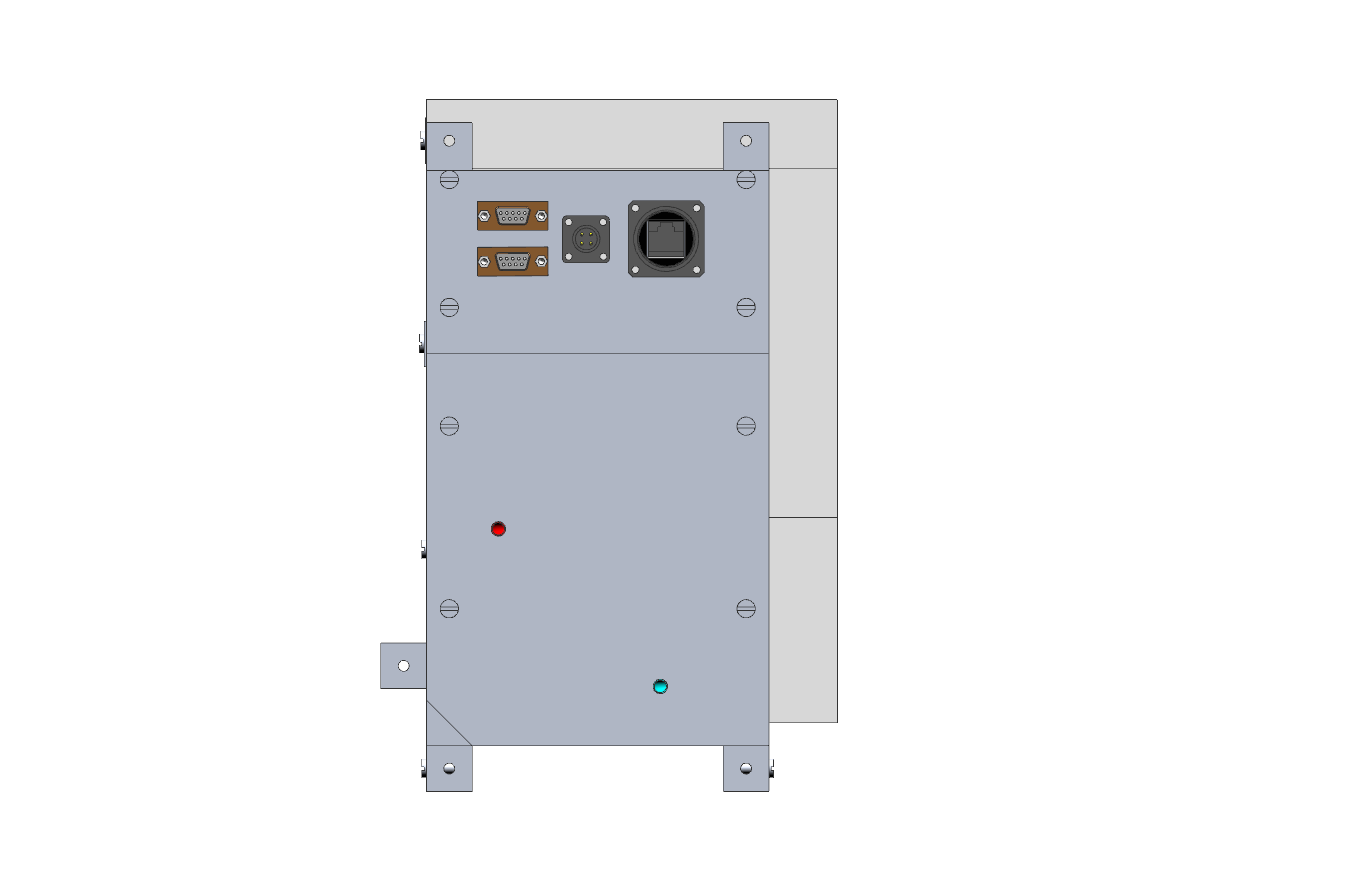
\includegraphics[width=1\textwidth]{4-experiment-design/img/Mechanical%/Panel_Front.png}
%    \caption{Front View of The Brain Where the Styrofoam Walls can be Identified.}
%    \label{brain_front}
%\end{figure}

\subsubsection{Pneumatic Subsystem}
\label{sec:4.4.5}

In order to be able to collect separated samples of air, a pneumatic subsystem has been developed. The schematics and components of this can be seen in Figure \ref{pneumatic_system}. The system is formed by almost $100$ components located inside The Brain and the AAC Box. 

In between these components, the same Sulfinert-treated stainless steel tubing as the ones used for the Inlet/Outlet pipes explained in Section \ref{subsec:pipes} have been chosen. According to the datasheet, the minimum suggested bend radius for the chosen diameter tube is $10.2\ cm$. Any bend sharper than this may cause the tubing to stretch, potentially creating active sites as the coating layer density decreases. For this reason, an auxiliary $90^\circ$ elbow interface has been added to perform all the required sharp curves to allocate all the components inside the volume-limited \emph{Brain}.

The schematic for the pneumatic system can be seen in Figure \ref{pneumatic_system}. The air is sucked from the outside through the inlet tube (No.1), turquoise in Figure \ref{pneumatic_system_cad}, and it goes through the filter (No.3) inside the pump (No.7). From here, it passes through the airflow sensor (No.11), which allows to monitor the flow rate, before changing to Level 2. Thereafter the air passes through the sensor box (No.15) which contains three pressure sensors before getting to the six stations manifold (No.19). It is in here where the air is directed to the desired bag (No.31) thanks to its dedicated solenoid valve (No.26).

When flushing the pneumatic system before each sampling period, the flushing valve (No.23) is opened so that the outlet of the system is open and new air runs through the main part of the pneumatic system. 

%\begin{figure}[H]
%    \centering
%    \begin{subfigure}[b]{0.48\textwidth}
%    \centering
%    \includegraphics[width=\textwidth]{4-experiment-design/img/Mechanical/ Pneumatic_System_Top_View_Level_1.png}
%    \caption{Top View of Level 1.}
%    \label{level_1_pneumatic_system_top_view}
%    \end{subfigure}
%    ~
%    \begin{subfigure}[b]{0.48\textwidth}
%    \centering
%    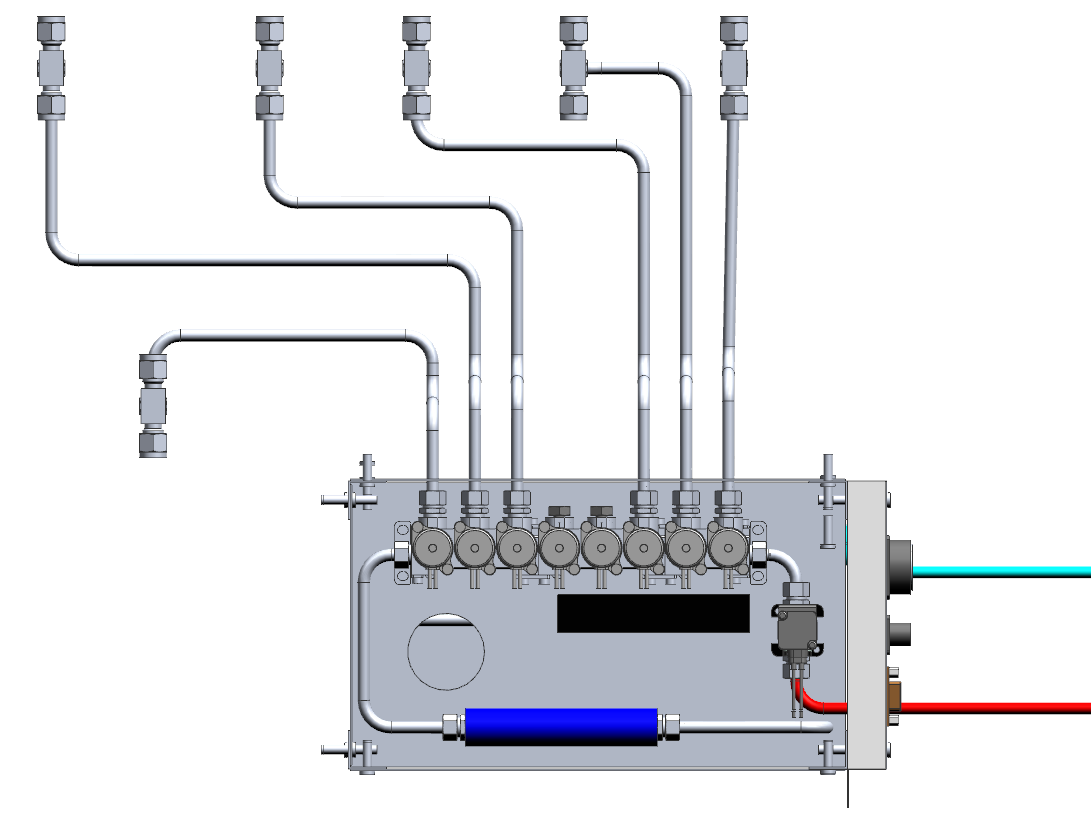
\includegraphics[width=\textwidth]{4-experiment-design/img/Mechanical/Pneumatic_System_Top_View_Level_2.png}
%    \caption{Top View of Level 2.}
%    \label{level_2_pneumatic_system_top_view}
%    \end{subfigure}
%    \caption{View Over the Pneumatic System.}
%    \label{fig:Pneumatic-system}
%\end{figure}

\begin{figure}[H]
    \centering
   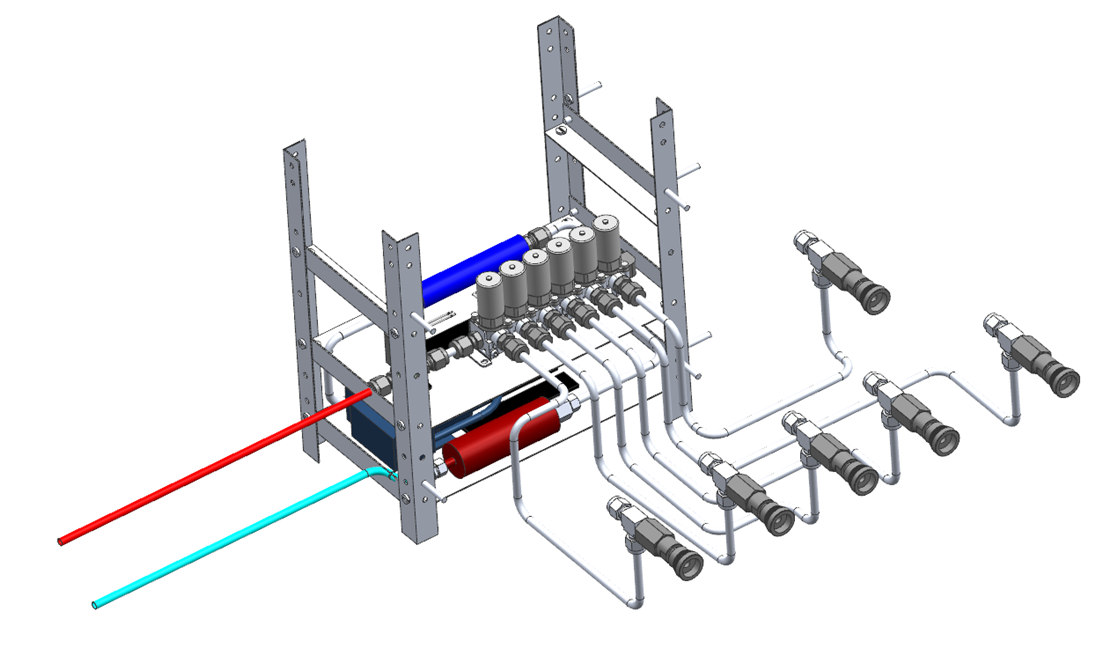
\includegraphics[width=0.8\textwidth]{4-experiment-design/img/Mechanical/Pneumatic_System.png}
   \caption{Pneumatic System Top View.}
    \label{pneumatic_system_cad}
\end{figure}

%\begin{figure}[H]
%    \centering
%    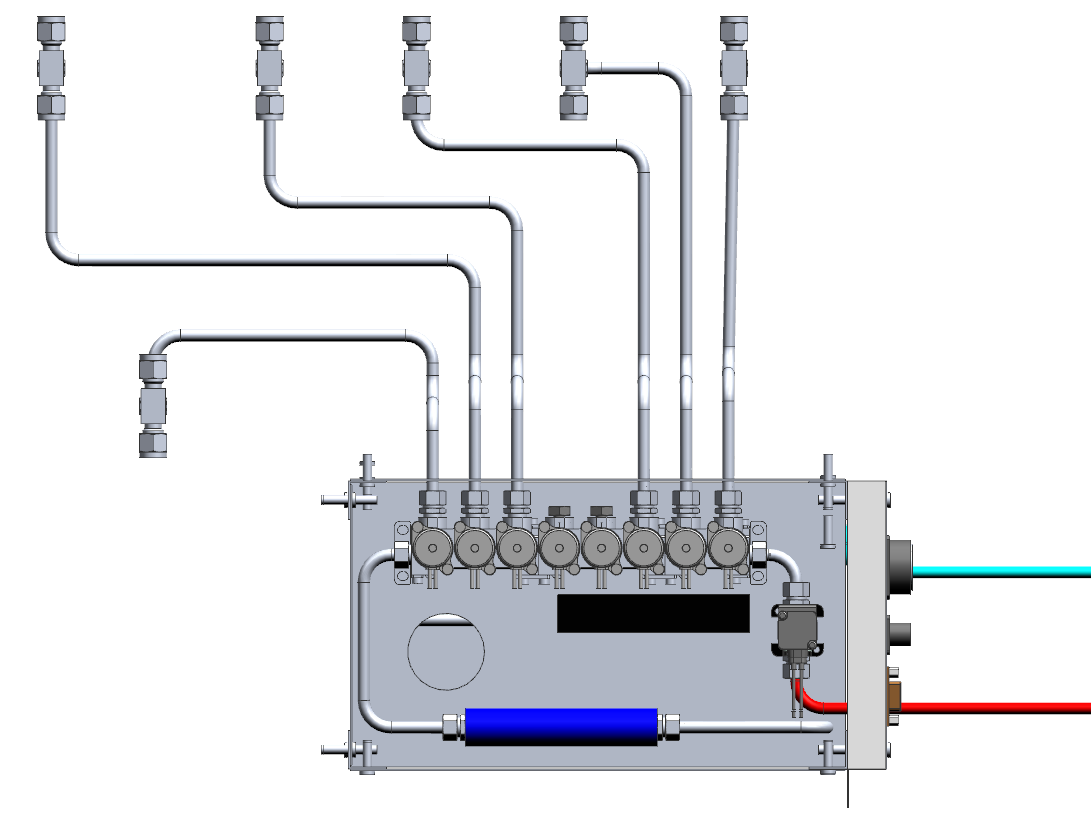
\includegraphics[width=0.8\textwidth]{4-experiment-design/img/Mechanical/Pneumatic_System_Top_View_Level_2.png}
%    \caption{Pneumatic System Top View of Level 2.}
%    \label{level_2_pneumatic_system_top_view}
%\end{figure}

% Figure with the diagram

\newpage
\begin{landscape}
\begin{figure}[H]
    \centering
    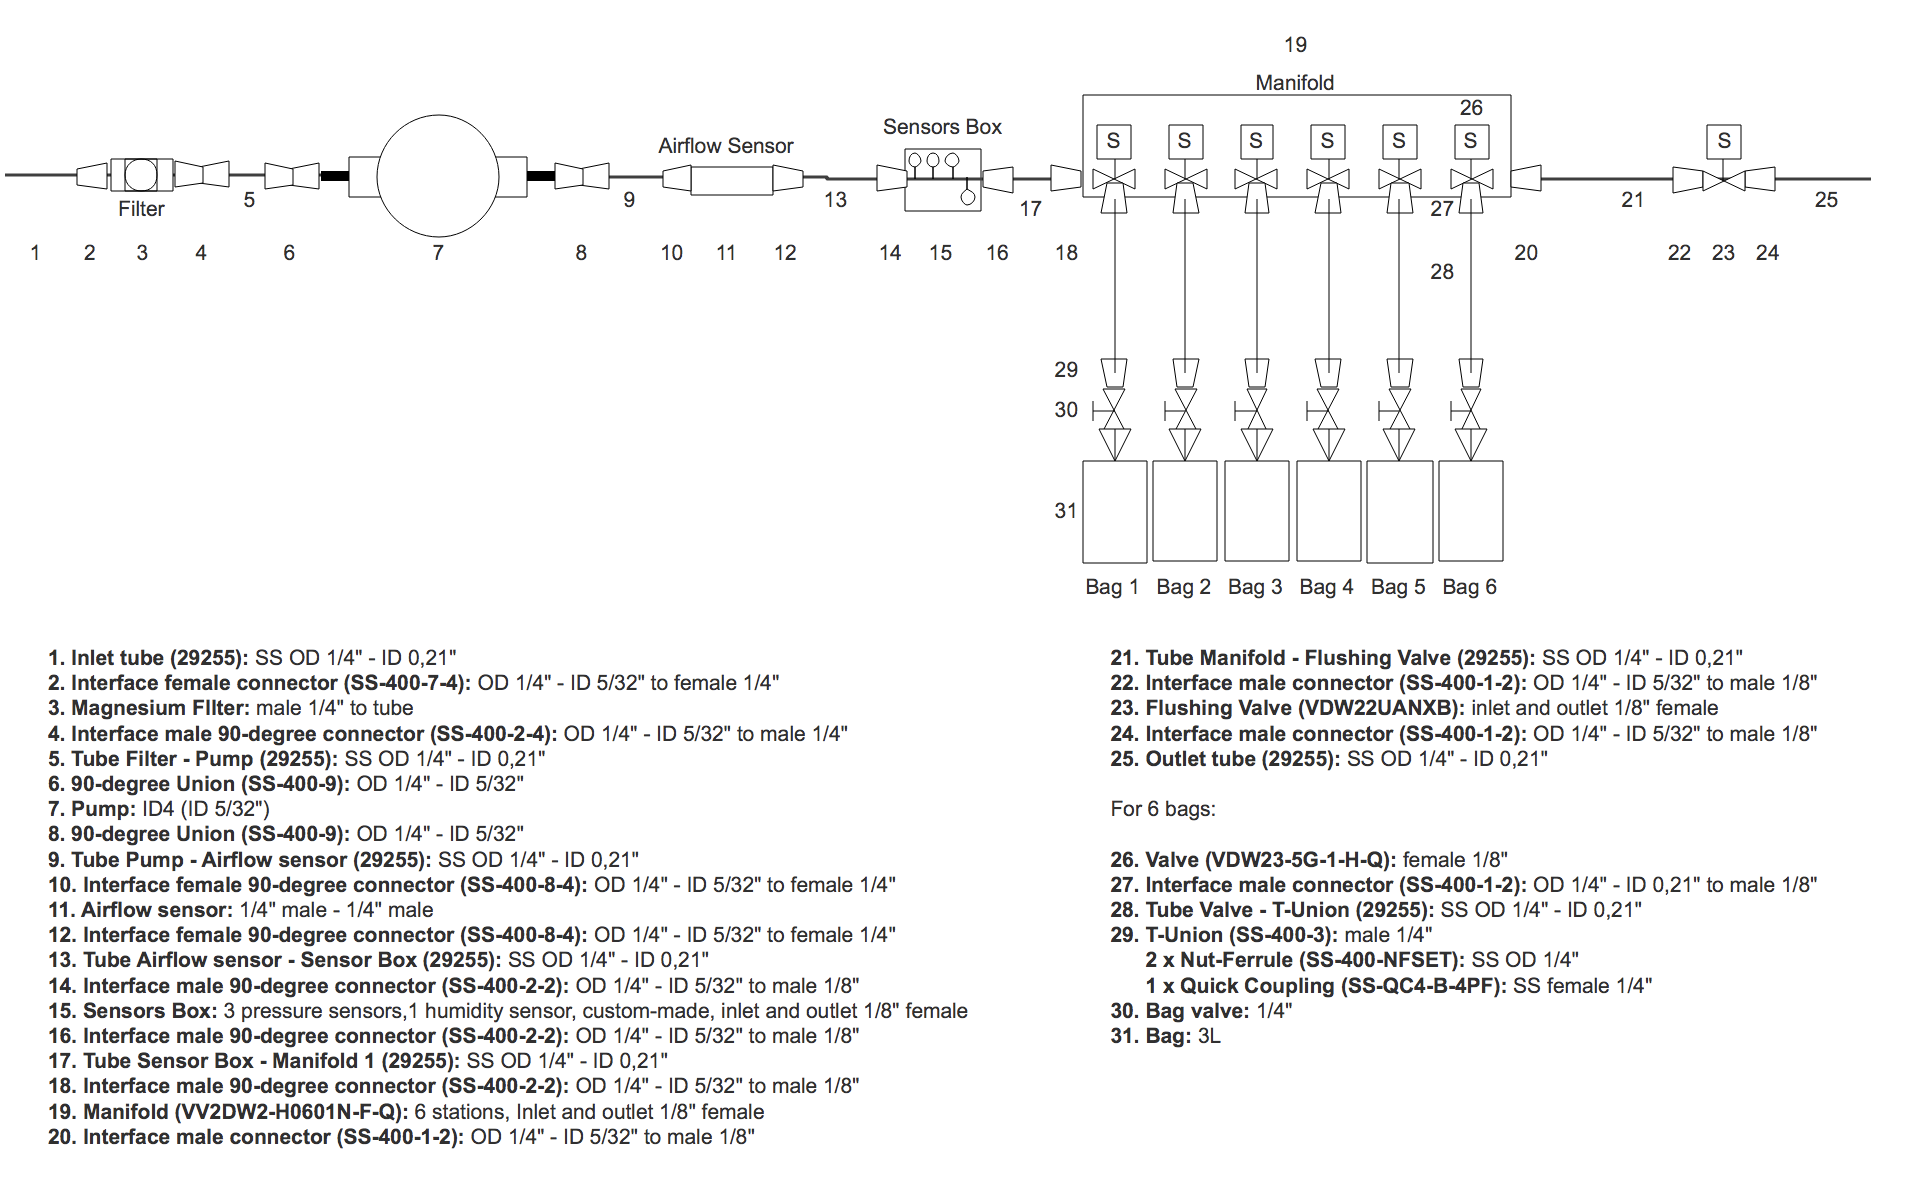
\includegraphics[width=1.45\textwidth]{4-experiment-design/img/Mechanical/AAC_Subsystem.png}
    \caption{AAC Pneumatic System Diagram and Components.}
    \label{pneumatic_system}
\end{figure}
\end{landscape}

\raggedbottom